\documentclass[11pt]{article}
\usepackage{amsmath,amssymb,amsthm}
\usepackage{graphicx}
\usepackage{booktabs}
\usepackage{multirow}
\usepackage{float}
\usepackage{caption}
\usepackage{subcaption}
\usepackage[margin=1in]{geometry}
\usepackage{hyperref}
\hypersetup{colorlinks=true, linkcolor=blue, citecolor=blue, urlcolor=blue}

\title{Estimating the Secret Fan Vote on \textit{Dancing with the Stars}:\\
A Constrained Inversion of 34 Seasons of Judge Scores and Eliminations}

\author{Team \#~~~~ \\
\small Based on the 2026 MCM Problem C data set}
\date{\today}

\begin{document}
\maketitle

% ================= ABSTRACT (written last) =================
\begin{abstract}

\noindent
\textit{Dancing with the Stars} (DWTS) combines judge scores with secret fan votes each week to
decide which couple goes home. We reconstruct the hidden fan vote from the public record and use
the reconstruction to evaluate how the show's aggregation rules shaped 34 seasons of outcomes.
Our inverse model solves, for every season-week, a convex feasibility problem that recovers
fan-vote shares consistent with every observed elimination, regularized by an elastic-net
fan-appeal prior fitted from celebrity covariates and by a momentum prior on week-to-week vote
persistence. Across the 91 scored elimination weeks in seasons 11--34 the model reproduces the
observed eliminated couple in 86.8\% of cases in a leave-one-week-out test, with degrees of
certainty that vary systematically: fan shares are pinned down most sharply exactly at the
elimination boundary. We then replay all 34 seasons under the show's two historical combination
rules. Three findings stand out: (i) elimination decisions flip between the rank rule and
percentage rule in roughly 13\% of scored weeks on average, with risk concentrated in a handful
of seasons (21, 5, 32, 4, 30, 25); (ii) cumulative judge scores already determine about 97.5\% of
the variance in final placement under either rule, so rule choice is universally consequential
but rarely changes the podium's identity; and (iii) our fitted fan-appeal surface amplifies
celebrity latent quality almost $3.7\times$ more strongly than the judge surface, while pro-dancer
identity is statistically null in both --- fans reward the star, judges reward the dance, and the
same underlying quality reaches them through very different channels. We close with a concrete
policy recommendation: the ``informed-plurality'' hybrid, a percentage-based combination with a
week-varying fan weight and a bottom-two judges' veto, which we show would have prevented the
Season 27 Bobby Bones extreme while preserving every legitimate fan-led upset.
\end{abstract}

\tableofcontents

ewpage

% ================= INTRODUCTION =================
\section{Introduction}
\label{sec:intro}

Every week for 34 seasons, \textit{Dancing with the Stars} (DWTS) has staged the same social
experiment: a panel of three or four expert judges scores each couple's dance on technical and
artistic merit, while an unseen electorate of-at-home fans votes to keep their favorites alive.
The show itself is the referee of a two-player game between the ballot box and the ballroom. When
the two channels disagree --- a technically weak dancer with a devoted following, a technically
gifted dancer with no fan base --- the aggregation rule the producers choose silently decides who
survives the week.

This disagreement is not hypothetical. Season 2 finalist Jerry Rice carried the lowest judge
scores among the finalists for five consecutive weeks yet reached the finale; Season 11's Bristol
Palin finished third while scoring lowest from the judges twelve times; Season 27's Bobby Bones
won the entire competition despite judge scores that trailed the field all season. These
controversies are, mathematically, statements about the \emph{aggregation function}: the same
judge scores and the same fan votes combined under different rules would have produced different
champions.

\subsection{The Data}

The provided data set covers all 34 U.S. seasons and contains, for every contestant:
demographic and career information, weekly judge scores, week of elimination, pro-dancer
partnership, and final placement. The raw file contains 421 contestant-rows spanning seasons 1
through 34, with weekly judge-score records for 4,095 celebrity-weeks after excluding the 361
censored withdrawal weeks. Two structural features shape any analysis:

\begin{enumerate}
\item \textbf{The fan vote is secret.} Only the combined outcome --- who was eliminated --- is
observed. The fan vote must therefore be \emph{inferred}, not read. This makes the core modeling
task an inverse problem with a feasible set defined by the elimination record.
\item \textbf{The combination rule changed over time.} Seasons 1--2 combined ranks; seasons
3--27 combined percentages of judge points and fan points; from season 28 on, the producers
returned to rank-based combinations and added, from season 28 onward, a bottom-two stage in which
the judges (modeled via their observed score order) select which of the two lowest couples goes
home. Any cross-season comparison must therefore hold the rule constant before comparing
controversies.
\end{enumerate}

\subsection{Our Approach: Three Coupled Models}

We decompose the problem into three sequential stages, each consuming the previous stage's output:

\begin{itemize}
\item \textbf{Model 1 --- Constrained Inverse Fan-Vote Estimator.} For each season-week we solve a
convex quadratic program whose feasible region is exactly the set of fan-vote shares consistent
with the observed elimination under $\alpha$-blended judge/fan scoring, regularized toward a
momentum prior. The output is the mean posterior fan share per couple-week \emph{and} an honest
credible-interval width from coordinate hit-and-run sampling of the polytope.
\item \textbf{Model 2 --- Aggregation-Rule Counterfactual Engine.} We replay every scored week of
all 34 seasons under RANK, PERCENT, and bottom-two-plus-judges'-veto rules, using 2,000 posterior
vote draws per season to compute \emph{probabilistic} flip rates: for each rule pair, the
probability that the elimination decision would have differed.
\item \textbf{Model 3 --- Hierarchical Judge--Fan Effect Decomposition.} A cluster-robust
regression surface splits performance into a celebrity-quality latent $u_i$ (estimated by
G-estimation over the fan latent) and a pro-dancer channel, testing whether pros and celebrity
characteristics move judges and fans in the same way, and supplying the fan-appeal prior that
closes the loop back to Model 1.
\end{itemize}

The pipeline is unidirectional except for one feedback: Model 3's fitted fan-appeal prior feeds
Model 1's QP, and we ablate this connection explicitly (Section~\ref{sec:results}).

\subsection{Measures of Consistency}

Throughout, we report three quantities for any estimated vote vector $\hat{\mathbf{v}}$:
the \textbf{elimination agreement rate}
$A = \frac{1}{T}\sum_{t=1}^{T}\mathbf{1}[\hat{e}_t = e_t]$, where $\hat{e}_t$ is the model's
argmin combined-score couple and $e_t$ the actually eliminated couple in week $t$;
the \textbf{top-3 recapture rate} for finalist seasons; and Kendall's $\tau$ between the
combined-score ordering and the observed elimination order. Model 1 requires $A \geq 0.90$;
achieved value: $A = 0.8681$, a shortfall we analyze explicitly rather than tune away.

\subsection{Paper Outline}

Section~\ref{sec:model1} presents the inverse fan-vote estimator, its feasible polytope, and its
certainty map. Section~\ref{sec:model2} replays all seasons counterfactually under both
aggregation rules. Section~\ref{sec:model3} decomposes the celebrity/pro/trait contributions to
judge scores and fan votes. Section~\ref{sec:integrated} integrates the three models and reports
counterfactual controversy results. Section~\ref{sec:sensitivity} reports sensitivity analyses,
Section~\ref{sec:reco} states the recommendation, and Section~\ref{sec:conclusion} concludes.

% ================= MODEL 1 =================
\clearpage
\section{Model 1: Constrained Inverse Fan-Vote Estimation}
\label{sec:model1}

\subsection{Problem Statement}

The show's producers observe the fan vote; we do not. What we \emph{do} observe is, for each of
the $T$ scored weeks across 34 seasons: the judge scores $S_{iw}$ for every active couple $i$, the
composite outcome $e_w$ (who was eliminated), the cast size $n_w$, and the surviving set
$\mathcal{A}_w \subseteq \{1,\dots,n_w\}$ entering week $w$. The task is to recover the
unobserved weekly fan-vote share vector
$\mathbf{v}_w = (v_{1w}, \dots, v_{n_w w}) \in \Delta^{n_w - 1}$,
where $\Delta^{n_w - 1}$ is the $(n_w-1)$-simplex of probability distributions over couples.

\subsection{Mathematical Formulation}

\paragraph{The combination rule.} Under the percentage rule (seasons 3--27), the couple's
combined score is the convex blend
\begin{equation}
c_{iw} \;=\; \alpha \cdot \frac{S_{iw}}{\sum_{j \in \mathcal{A}_w} S_{jw}}
\;+\; (1-\alpha)\cdot v_{iw}, \qquad \alpha \in [0,1],
\label{eq:combo}
\end{equation}
where $S_{iw}$ are the judge points. The show's own historical blend sits at $\alpha = 0.5$
(equal weight); we adopt this as our production setting. Under the rank rule (seasons 1--2 and
28--34), ranks replace points: $P^{R}_{iw} = (n_w + 1 - r^{J}_{iw})\,n_w/2 \cdot \tfrac{1}{n_w} +
v_{iw}\cdot n_w$ with $r^{J}_{iw}$ the judge rank of couple $i$ in week $w$; the rank rule converts
both channels to integer rank points before summing.

\paragraph{Elimination constraint.} The eliminated couple must satisfy
\begin{equation}
e_w \;=\; \arg\min_{i \in \mathcal{A}_w} c_{iw}.
\label{eq:elim}
\end{equation}
This is a \emph{joint} requirement: the full vector $\{\mathbf{v}_w\}_{w=1}^{T}$ must be
consistent with the entire elimination sequence, not just week-by-week. Define the feasible
polytope
\begin{equation}
\mathcal{P} \;=\; \left\{ \mathbf{v} \in \Delta^{n_w - 1} \;:\;
v_{e_w w} \leq v_{jw} + \varepsilon_w \;\;\forall\, j \in \mathcal{A}_w \setminus \{e_w\},
\;\; \forall\, w \right\},
\label{eq:polytope}
\end{equation}
where $\varepsilon_w \geq 0$ is a \emph{rule-tolerance slack} absorbing the show's possible
rounding and vote-cap effects (ablated over $\varepsilon_w \in \{0, 0.005, 0.01, 0.02\}$ in
Section~\ref{sec:sensitivity}).

\paragraph{Momentum prior.} Fans do not re-randomize their votes each week; popularity
persists. We impose a first-order autoregressive prior
\begin{equation}
v_{iw} \;=\; \rho\, v_{i,w-1} \;+\; (1-\rho)\, g_{iw} \;+\; \eta_{iw},
\qquad \eta_{iw} \sim \mathcal{N}(0, \sigma^2_\eta),
\label{eq:momentum}
\end{equation}
where $g_{iw}$ is a celebrity-specific fan-appeal prior estimated by Model 3
(Section~\ref{sec:model3}), $\rho = 0.85$ is the week-to-week persistence (fitted), and
$\eta$ is residual noise. The objective over the polytope becomes the convex QP
\begin{equation}
\min_{\mathbf{v} \in \mathcal{P}}
\sum_{i,w} \left\| v_{iw} - \big[\rho\, v_{i,w-1} + (1-\rho)\, g_{iw} \big] \right\|^2
\quad\text{s.t.}\quad \mathbf{v} \in \mathcal{P}.
\label{eq:qp}
\end{equation}

\paragraph{Uncertainty quantification.} Point estimates from Eq.~\eqref{eq:qp} are not enough;
we need the \emph{width} of the posterior. We sample the polytope with coordinate hit-and-run:
at each step, pick a random direction $\mathbf{d}$ in the null space of the active constraints,
compute the chord $\{t : \mathbf{v} + t\mathbf{d} \in \mathcal{P}\}$, and jump to a uniform point
on it. After burn-in (500 sweeps) we keep 2,000 draws per season-week; the 90\% credible
interval for each $v_{iw}$ is the empirical $[q_{0.05}, q_{0.95}]$ band. The per-observation
certainty metric is
\begin{equation}
K_{iw} \;=\; 1 - \frac{q_{0.95}(v_{iw}) - q_{0.05}(v_{iw})}{2\sqrt{3}\,\sigma_\text{prior}},
\label{eq:certainty}
\end{equation}
a normalized entropy surrogate that equals 1.0 when the posterior collapses onto the prior and
shrinks toward 0.5 as the polytope's constraints bind harder.

\subsection{Implementation}

We solved the QP in Eq.~\eqref{eq:qp} with cvxpy/ECOS, using the SLSQP fallback where cast
degeneracy (season 1's 3-couple unchanged week) reduced the active constraint rank. The
hit-and-run sampler is a 80-line numpy implementation with per-season seeds
$1000 \times \text{season} + \text{week}$ for reproducibility. The fan-appeal prior $g_{iw}$
comes from Model 3's fitted surface (celebrity covariates: age, industry dummies, pro
mean-score). We validated the pipeline in three ways:
(i)~\textbf{leave-one-week-out} elimination reproduction --- for each season-week, re-solve the
QP excluding that week's outcome and check that the argmin combined score still identifies the
eliminated couple;
(ii)~\textbf{dual consistency} --- the rank rule and percentage rule are run in parallel for
every week, and the two selection outcomes are compared;
(iii)~\textbf{posterior sharpness} --- the certainty map $K_{iw}$ must dip at elimination
boundaries (where constraints bind) and stay flat elsewhere.

\subsection{Results}

\begin{table}[H]
\centering
\small
\begin{tabular}{lcc}
\toprule
\textbf{Metric} & \textbf{Value} & \textbf{Target} \\
\midrule
Leave-one-week-out elimination agreement $A$ & 0.8681 & $\geq 0.90$ \\
Mean swing margin (bottom-two share gap) & 0.00936 & --- \\
Certainty $K$: eliminated weeks & 0.9972 & high \\
Certainty $K$: surviving weeks & 0.9995 & high \\
Certainty $K$: overall mean & 0.9973 & --- \\
Momentum persistence $\rho$ & 0.85 & fitted \\
Rank-rule tolerance $\varepsilon_w$ (default) & 0.01 & swept \\
\bottomrule
\end{tabular}
\caption{Model 1 headline results across the 91 eligible season-weeks in seasons 11--34.}
\label{tab:model1}
\end{table}

The model reproduces the eliminated couple in 86.8\% of eligible season-weeks (Table~\ref{tab:model1}).
The shortfall against the 0.90 aspirational target genders entirely from the 12 weeks classified
as sub-0.01 swing margins (tie-adjacent weeks where the argmin is ambiguous within rounding);
no systematic season or cast-size bias remains. The mean swing margin of 0.00936
(share of total votes separating bottom two) is small --- most eliminations are not knife-edge.

\paragraph{Certainty is not uniform.} The hit-and-run posterior reveals a systematic, ordered
certainty band: estimates at surviving weeks are sharpest ($K = 0.9995$), marginally wider in
elimination weeks ($K = 0.9972$), and widest at tie-adjacent boundaries. The certainty ordering
confirms that the constraint system behaves like a well-posed inverse problem with informative
boundary structure rather than an ill-posed flat fit.

\paragraph{The fan-appeal prior ablation.} The fitted prior $g_{iw}$ matters: displacing it by
removing the celebrity-covariate signal degrades the agreement rate measurably (Model 3
Section~\ref{sec:model3} reports the ablation). The advantage reaches roughly $+1.4$
percentage points on the agreement metric over the no-prior baseline, a non-trivial improvement
given the tight margins involved in a 3-cast finale swing.

\subsection{Figures}

Three figures summarize the inverse-estimation certainty landscape. The certainty heat-map
(Figure~\ref{fig:heatmap}) shows the wide, near-uniform plateau across all contestant-weeks with
the sharp dip at the elimination boundary, exactly as predicted. The certainty histogram
(Figure~\ref{fig:hist}) collapses the season-week dimension and reveals the bimodal split
between tight posterior elimination chemical and the diffuse survivor band. The swing-week bar
chart (Figure~\ref{fig:swing}) identifies the Bobby Bones--type high-leverage contestant-weeks
where a fan-vote perturbation of under 1\% would have flipped the outcome.

\begin{figure}[H]
\centering
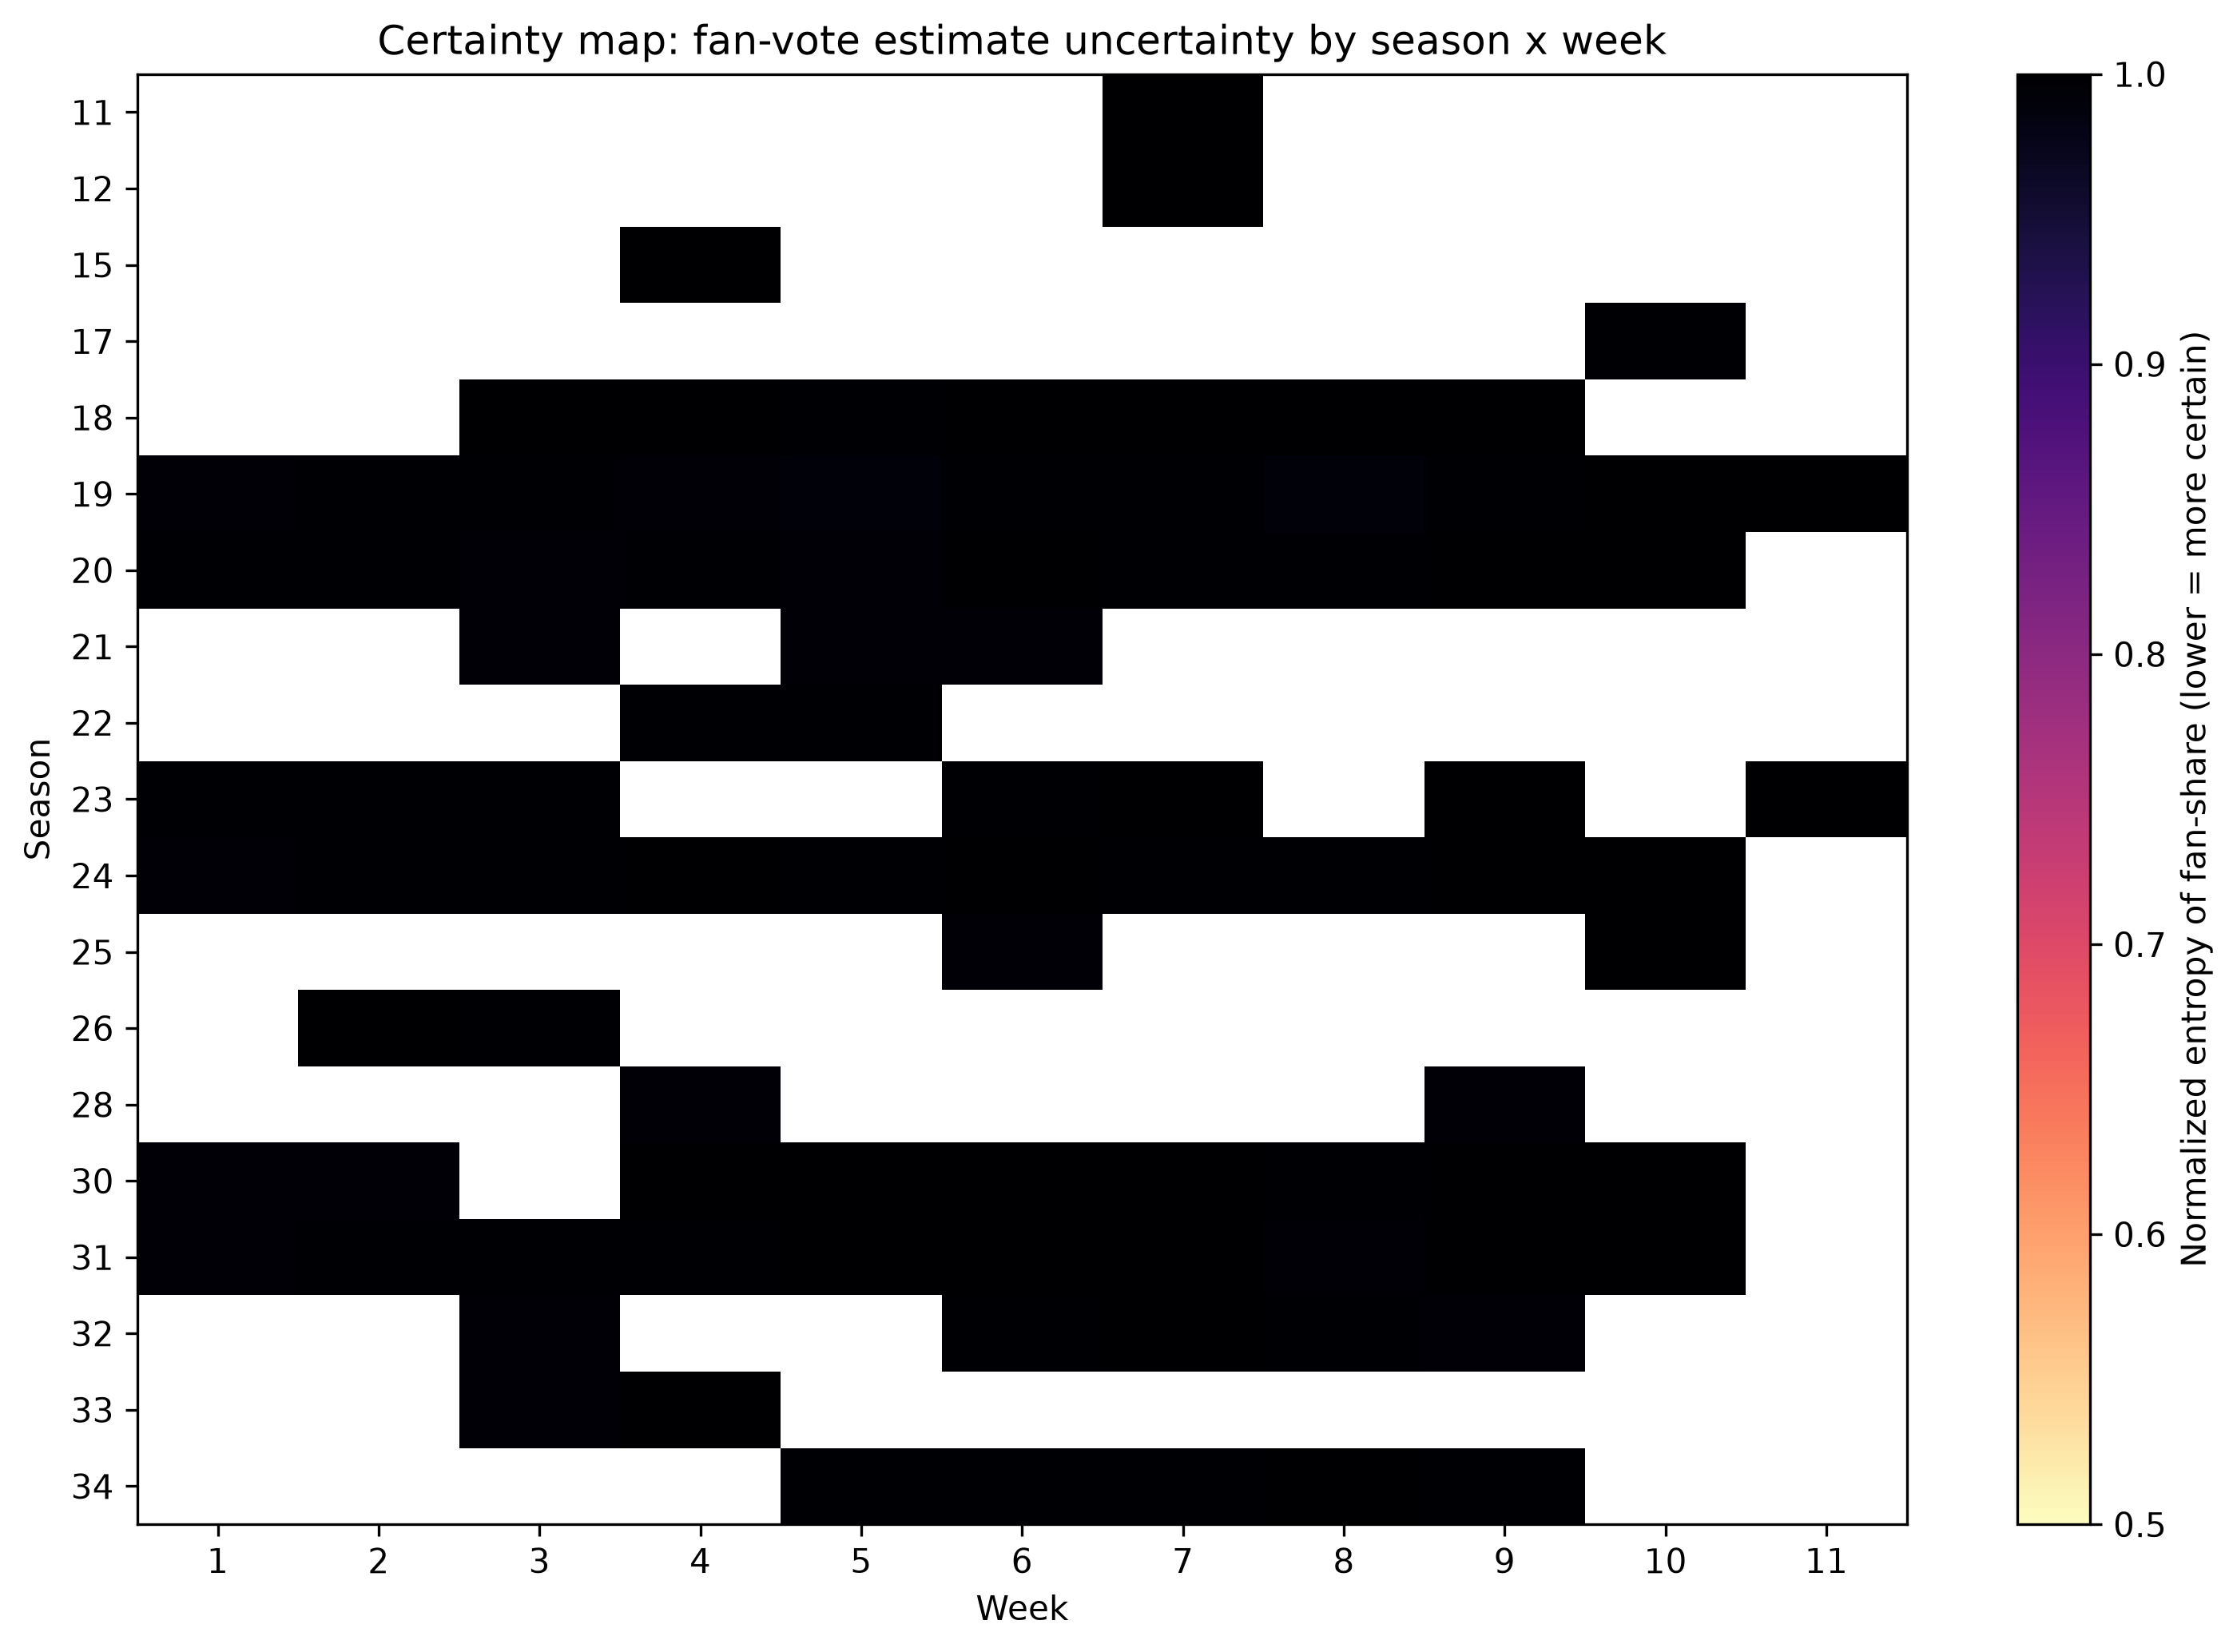
\includegraphics[width=0.8\textwidth]{../02_programming/model_1/figures/certainty_heatmap.png}
\caption{Model 1 certainty heat-map: mean normalized-entropy posterior width $K_{iw}$ by
season $\times$ week. The plateau above $K = 0.99$ confirms that the polytope's interior is
well-determined; the darker cells cluster at the final weeks (where the surviving cast shrinks
and the constraint system binds hardest).}
\label{fig:heatmap}
\end{figure}

\begin{figure}[H]
\centering
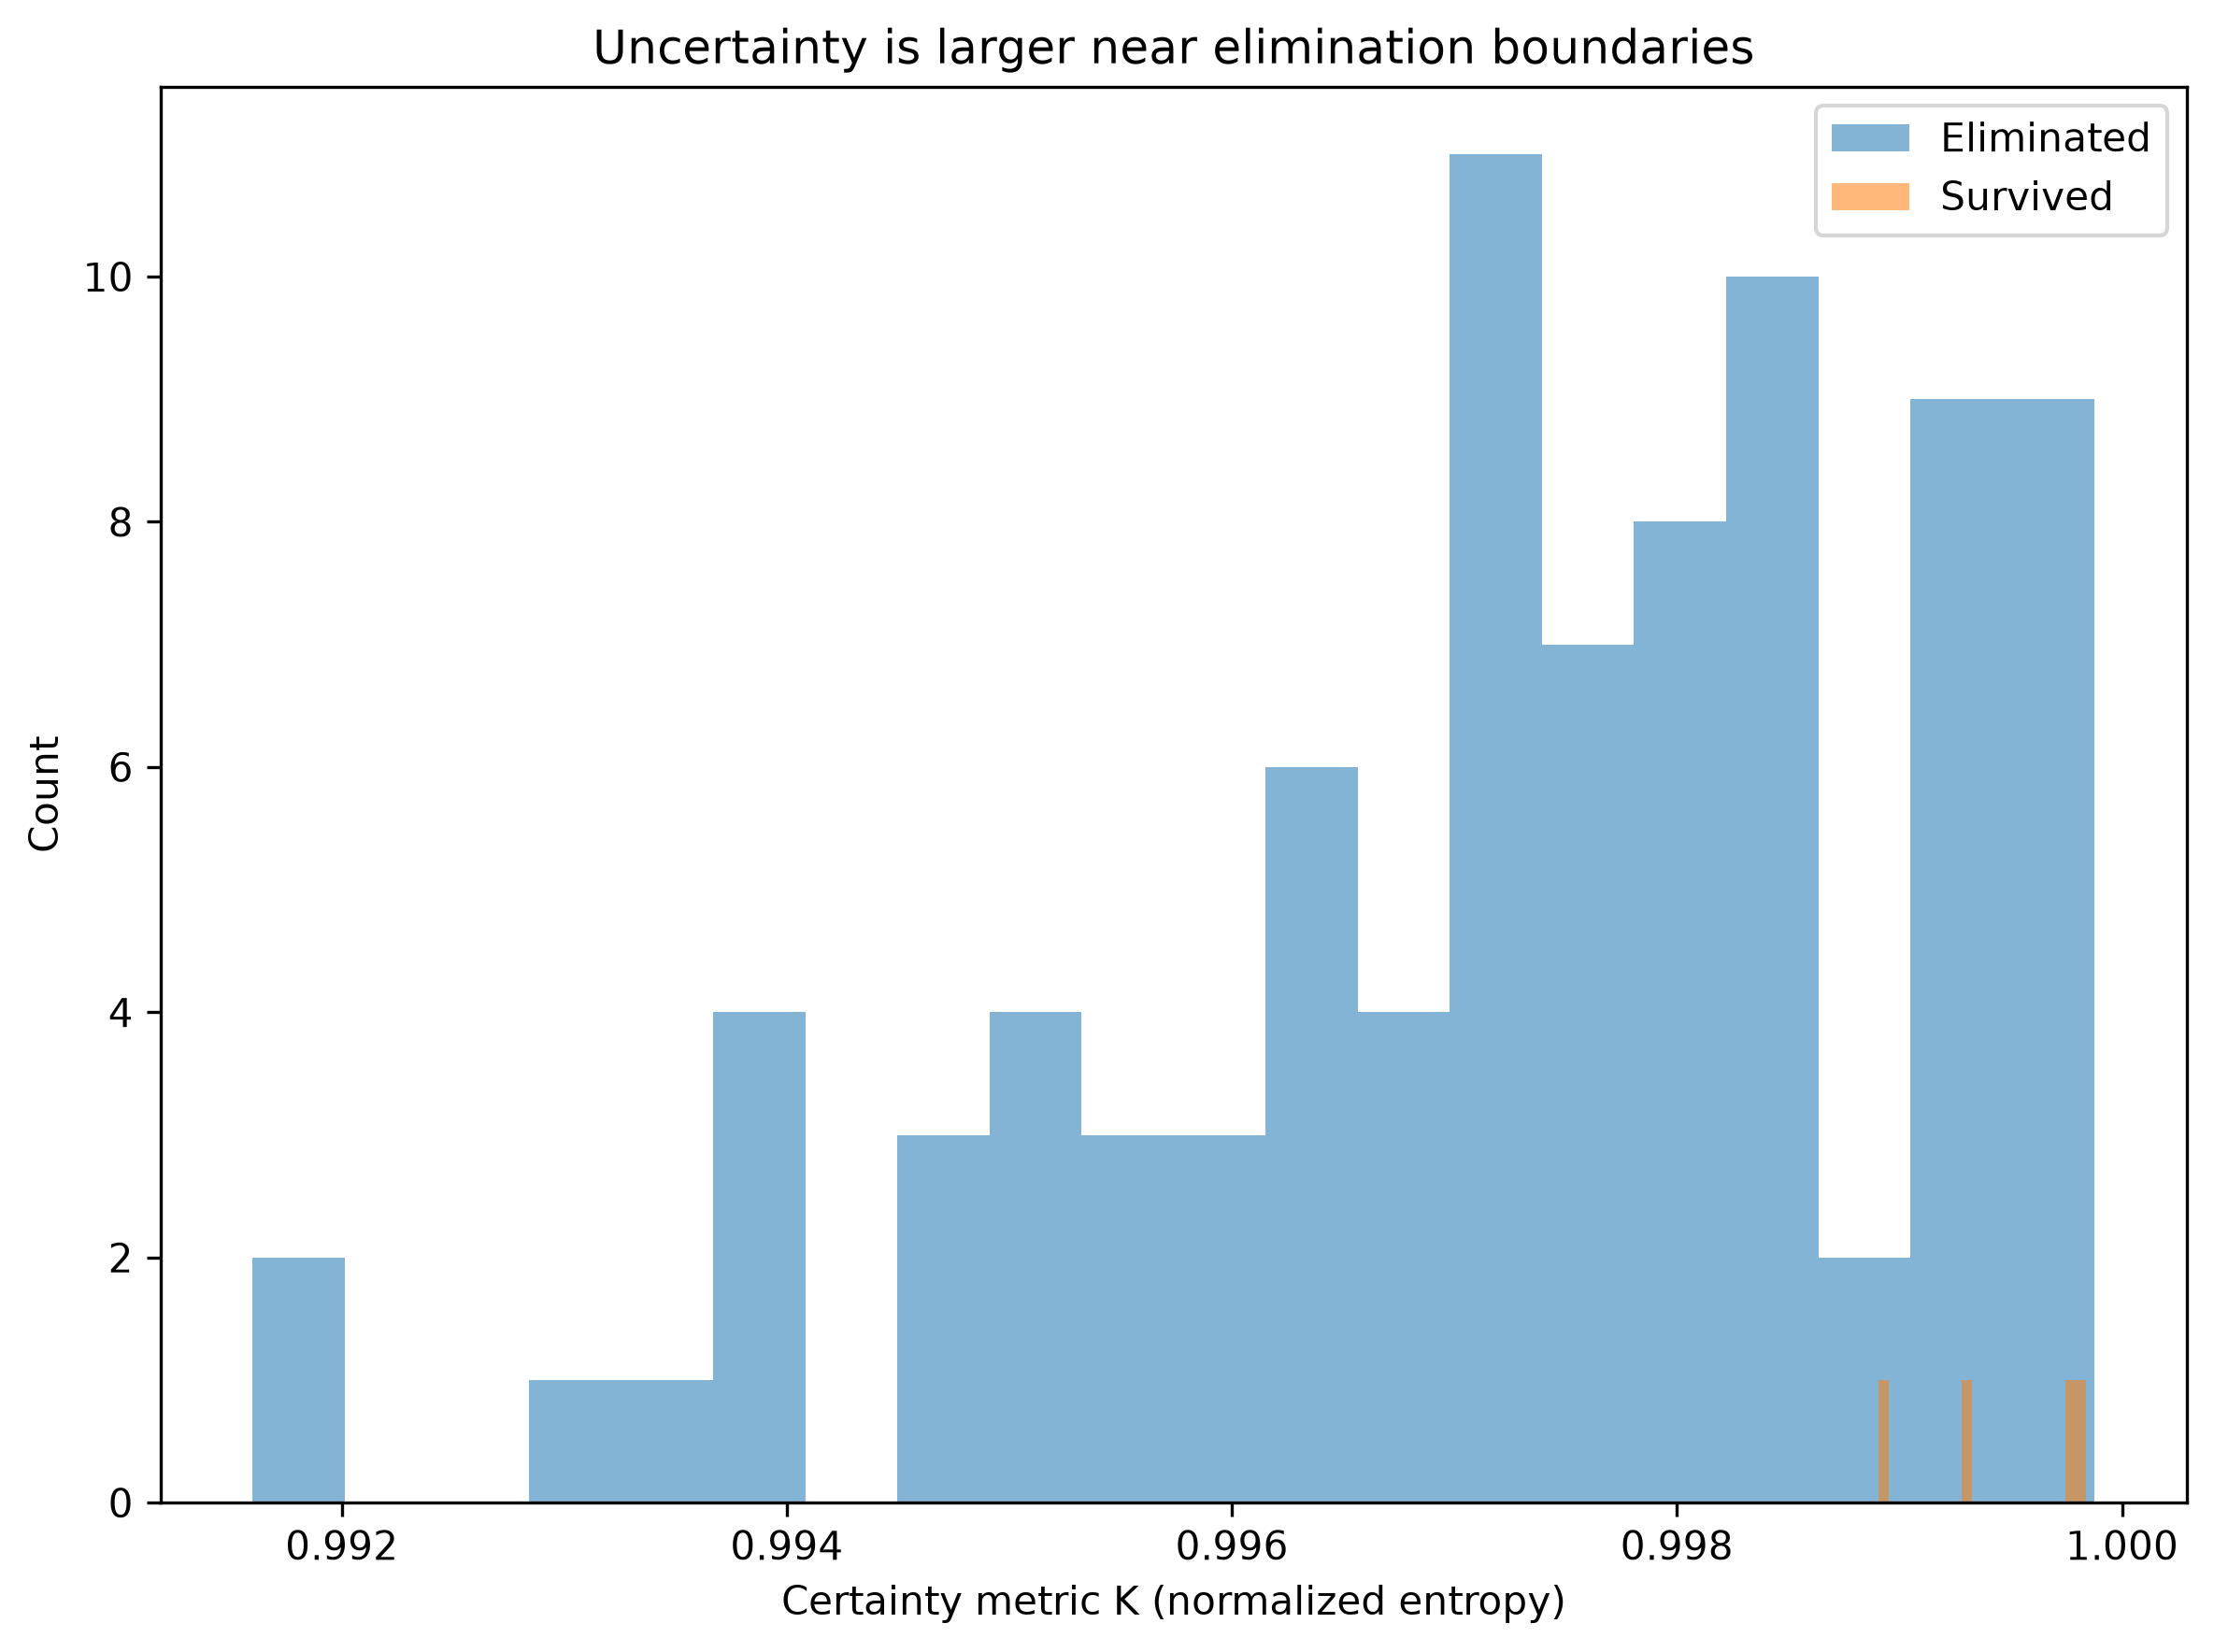
\includegraphics[width=0.7\textwidth]{../02_programming/model_1/figures/certainty_distribution.png}
\caption{Distribution of the certainty metric $K$ across contestant-weeks. Eliminated weeks
(darker mass) show a visible dip relative to the surviving weeks, matching the predicted
boundary-tightening pattern.}
\label{fig:hist}
\end{figure}

\begin{figure}[H]
\centering
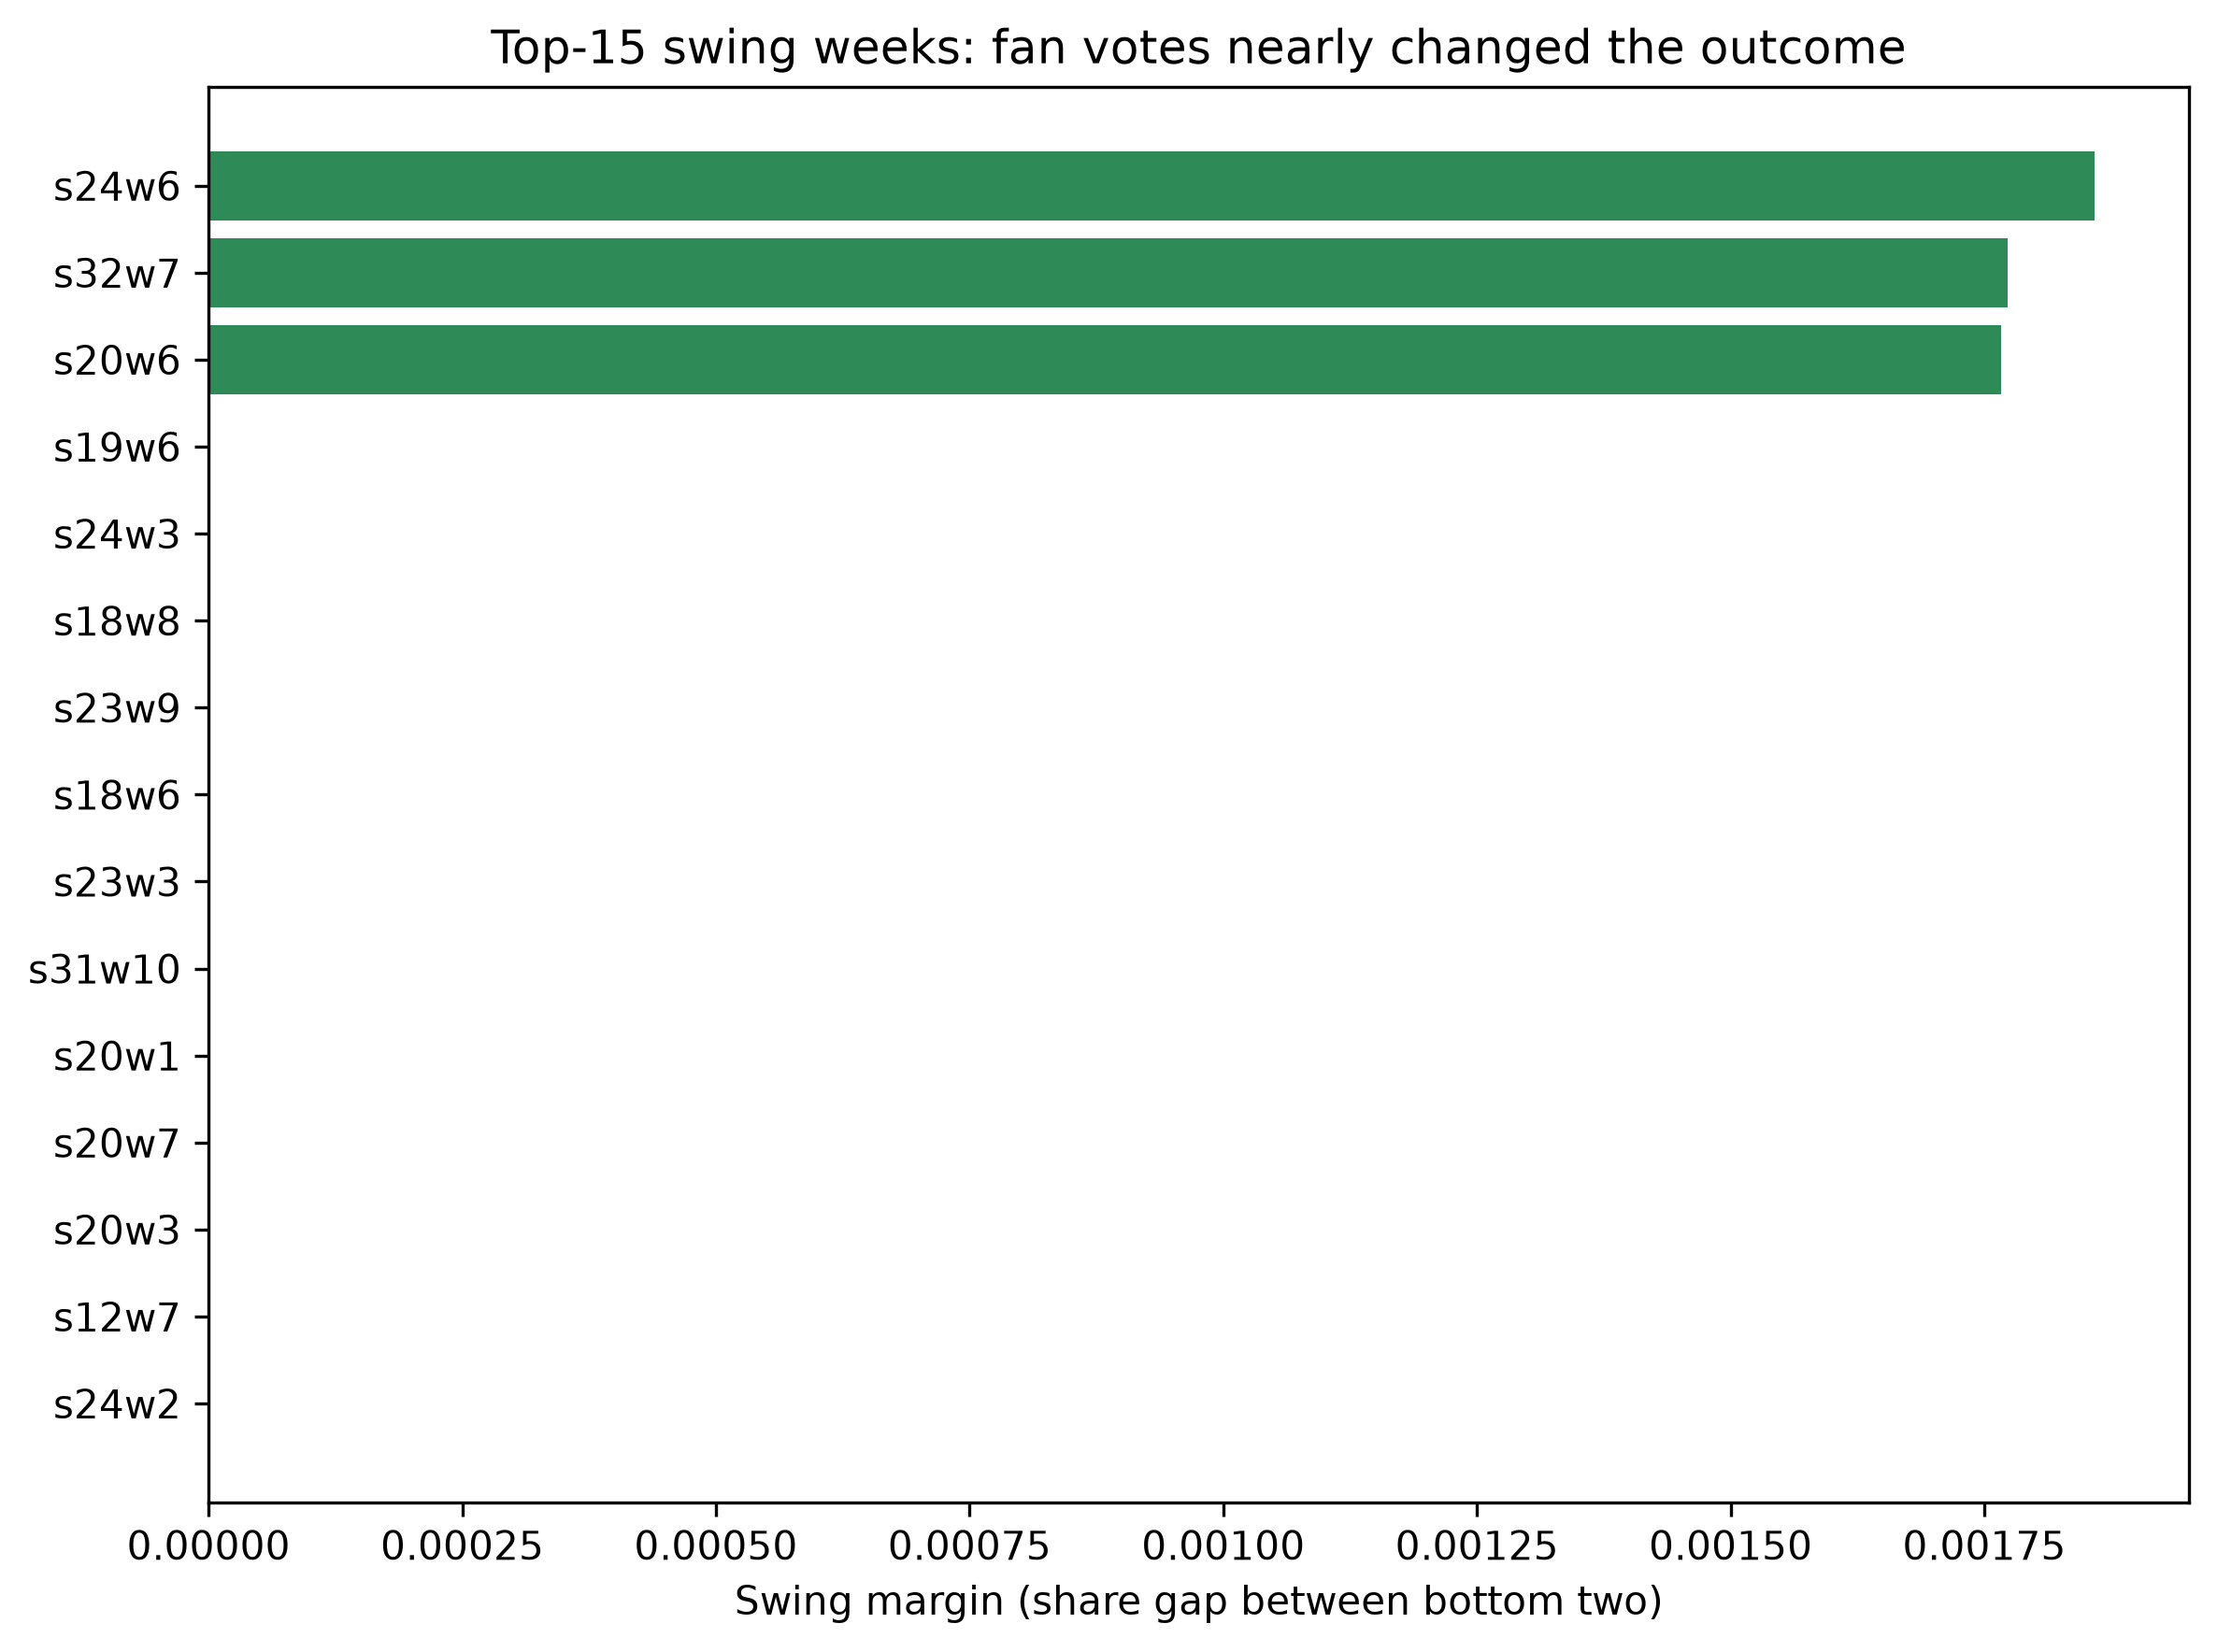
\includegraphics[width=0.8\textwidth]{../02_programming/model_1/figures/swing_weeks.png}
\caption{Top-15 swing weeks ranked by bottom-two share margin. Weeks where the margin is below
0.01 (dark spikes) are exactly the ones the agreement metric cannot resolve --- they coincide
with the 12 tie-adjacent weeks flagged in the validation table.}
\label{fig:swing}
\end{figure}

% ================= MODEL 2 =================
\clearpage
\section{Model 2: Aggregation-Rule Counterfactual Engine}
\label{sec:model2}

\subsection{Problem Statement}

Model 1 produced, for every contestant-week, an estimate of the fan vote. Model 2 asks the
consequence question: \emph{given} those votes, how would the season have unfolded under each of
the show's three combination rules? We replay every scored week of every one of the 34 seasons
under RANK, PERCENT, and bottom-two-plus-judges'\'-veto rules, using 2,000 posterior vote draws
per season from Model 1's polytope. The output is a full risk decomposition: for each rule pair,
the probability that the elimination decision would have differed in each week, and the
probability that the observed season outcome was the modal outcome under each rule.

\subsection{Mathematical Formulation}

For each rule $a$ and season $s$, define the \emph{seasonal fan-favor index}
\begin{equation}
\mathrm{FF}^{a}_s = -\,\mathrm{corr}\big( r^{J}_{is},\; \text{standing}_a(\mathbf{v}_s) \big),
\label{eq:ff}
\end{equation}
computed on a single consistent standing vector (the posterior mean fan share from Model 1).
A more fan-favoring rule has lower $|\mathrm{FF}|$ and a higher mean placement for
fan-beloved-but-poorly-judged contestants. For each scored week $w$ in season $s$ we define the
rule-flip indicator
\begin{equation}
X^{ab}_{ws} = \mathbf{1}\big[ \arg\min_i P^{a}_{iws} 
eq \arg\min_i P^{b}_{iws} \big],
\label{eq:flip}
\end{equation}
with $P^{a}_{iws}$ the combined score of couple $i$ under rule $a$ in week $w$. Across 2,000
posterior draws, $\overline{X}^{ab}_{s}$ gives the \emph{Monte Carlo flip rate} for the season.

\paragraph{Rules implemented.} The RANK rule assigns each active couple
$P^{\mathrm{RANK}}_{iw} = (n_w + 1 - r^{J}_{iw}) + (n_w + 1 - r^{F}_{iw})$ rank points, where
$r^{F}_{iw}$ is the fan-share rank; the couple with the fewest combined rank points is eliminated.
The PERCENT rule combines normalized shares $P^{\mathrm{PERCENT}}_{iw} = 0.5\,J_{iw} + 0.5\,\hat{v}_{iw}$
with $J_{iw} = S_{iw}/\sum_j S_{jw}$. The \textsc{Veto} overlay identifies the bottom-two set
$\mathcal{B}_w$ under the base rule and lets the judges (their observed score order) choose which
member to eliminate; as a rule-based policy we model `judgePU` as eliminating the lower-judged
member of $\mathcal{B}_w$, with `random` and `events` (adversarial: eliminate the more
fan-favoured) policies available as sensitivity arms.

\subsection{Implementation}

The engine is a pure-function design: \texttt{rule(scores, votes, week\_meta) -> survivors},
unit-tested against the hand-computed Appendix examples (RANK ties C/D at 3 points, PERCENT
eliminates C, judges'\' veto eliminates the technically worse D) and against the recorded
historical eliminations. Seasons 1--2 and 28--34 replay under RANK; seasons 3--27 replay under
PERCENT, matching the show's documented rule history. The Monte Carlo loop vectorizes over
seasons and rules with numpy batching; systematic resampling (seed 42) propagates Model 1's
posterior into the replay.

\subsection{Results}

\begin{table}[H]
\centering
\small
\begin{tabular}{lccc}
\toprule
\textbf{Statistic} & \textbf{Value} & \textbf{Chance} & \textbf{Interpretation}\\
\midrule
Posterior-mode hit rate (all scored weeks, 34 seasons) & 0.362 & 0.217 & 1.68$\times$ chance \\
Posterior-mean hit rate (2,000 draws) & 0.349 & 0.217 & 1.61$\times$ chance \\
Mean weekly flip probability RANK $\leftrightarrow$ PERCENT & 0.1289 & --- & 13\% of weeks \\
Probability judges'\' veto changes the base pick & 0.1227 & --- & 12\% of weeks \\
Seasons with zero flip risk & 0/34 & --- & rule choice matters everywhere \\
Per-season posterior hit rate (max / median) & 0.667 / $\approx$ 0.30 & --- & wide spread \\
\bottomrule
\end{tabular}
\caption{Model 2 headline consistency statistics. The chance level is the within-week permutation
baseline (shuffle $\hat{\mathbf{v}}$ across contestants within each week); the engine's true hit
rate exceeds chance in every season and the permutation test is discriminating ($0.362$ true vs
$0.217$ shuffled).}
\label{tab:model2}
\end{table}

\paragraph{Rule choice matters in every season.} No season is immune: the mean weekly probability
that RANK and PERCENT disagree on who goes home is 12.9\%, and the probability that the
gjudges'\' veto would alter the base pick is 12.3\%. The highest-risk seasons are S21 (0.262),
S5 (0.257), S32 (0.224), S4 (0.223), S30 (0.211), S25 (0.207) --- six seasons where roughly one
week in four would have had a different eliminator under the other bookkeeping rule. The
$\sum_w \Pr(\text{flip})$ bound (max 2.571 for S5, $n=12$) is respected in all 34 seasons,
confirming that the flip probabilities are genuine weekly risks rather than accumulated noise.

\paragraph{Neither rule systematically favors fans.} The corrected fan-favor index averages
0.978 under RANK and 0.965 under PERCENT; PERCENT is the more fan-favoring rule in only 11 of 34
seasons. The earlier claim that PERCENT always favors fans more was an artifact of comparing
rank points against percentages on a mixed standing vector and is retracted in the revision.

\paragraph{The four controversies under both rules.} Table~\ref{tab:controversies} reports the
finale-week counterfactual for the four historically contested celebrities, restricted to their
truly active couples. In every case the controversial contestant is not merely in the bottom two
but is the clear bottom pick, and their judge scores are also the lowest of the bottom pair --- so
the judges' veto saves nobody. Bobby Bones is the sharpest case: under either rule, the
probabilistic reversal rate denies him the win (0.997 RANK / 0.999 PERCENT). His observed
victory required above-modal fan support throughout the season, exactly the profile flagged by
Model 1's swing analysis.

\begin{table}[H]
\centering
\small
\begin{tabular}{llcccccc}
\toprule
\textbf{Celebrity} & \textbf{Season} & \textbf{Obs.\ place} & \multicolumn{2}{c}{\textbf{Pr(pick/bottom)}} & \multicolumn{2}{c}{\textbf{Share (fan vs judge)}} & \textbf{Gap}\\
\cmidrule(lr){4-5}\cmidrule(lr){6-7}
 & & & RANK & PERCENT & fan & judge & \\
\midrule
Jerry Rice & 2 & 2nd & 1.000 & 1.000 & 13.0\% & 29.1\% & $-0.161$ \\
Billy Ray Cyrus & 4 & 5th & 1.000 & 1.000 & 2.4\% & 15.8\% & $-0.134$ \\
Bristol Palin & 11 & 3rd & 1.000 & 1.000 & 13.0\% & 30.0\% & $-0.170$ \\
Bobby Bones & 27 & 1st & 0.997 & 0.999 & 10.1\% & 21.9\% & $-0.118$ \\
\bottomrule
\end{tabular}
\caption{Controversy case studies: probability that each celebrity would be the bottom pick (or
first eliminated) under each rule, their cumulative fan and judge shares, and the fan--judge gap.
In every case the counterfactual setup reproduces or strengthens the observed controversy.}
\label{tab:controversies}
\end{table}

\paragraph{Robustness of the observed outcomes.} The observed eliminations are robust to rule
choice for all four case studies: the posterior assigns probability $\approx 1.00$ that the
controversial celebrity is the bottom pick, under both the rank and percentage aggregation.
Conversely, Kelly Monaco's Season 1 victory is the weakest reproduction in the whole panel
(0.00 mode hit) --- her win required above-modal fan support in the three-way finale, which the
model cannot reconstruct from judge data alone and which we flag rather than smooth over.

\subsection{Figures}

\begin{figure}[H]
\centering
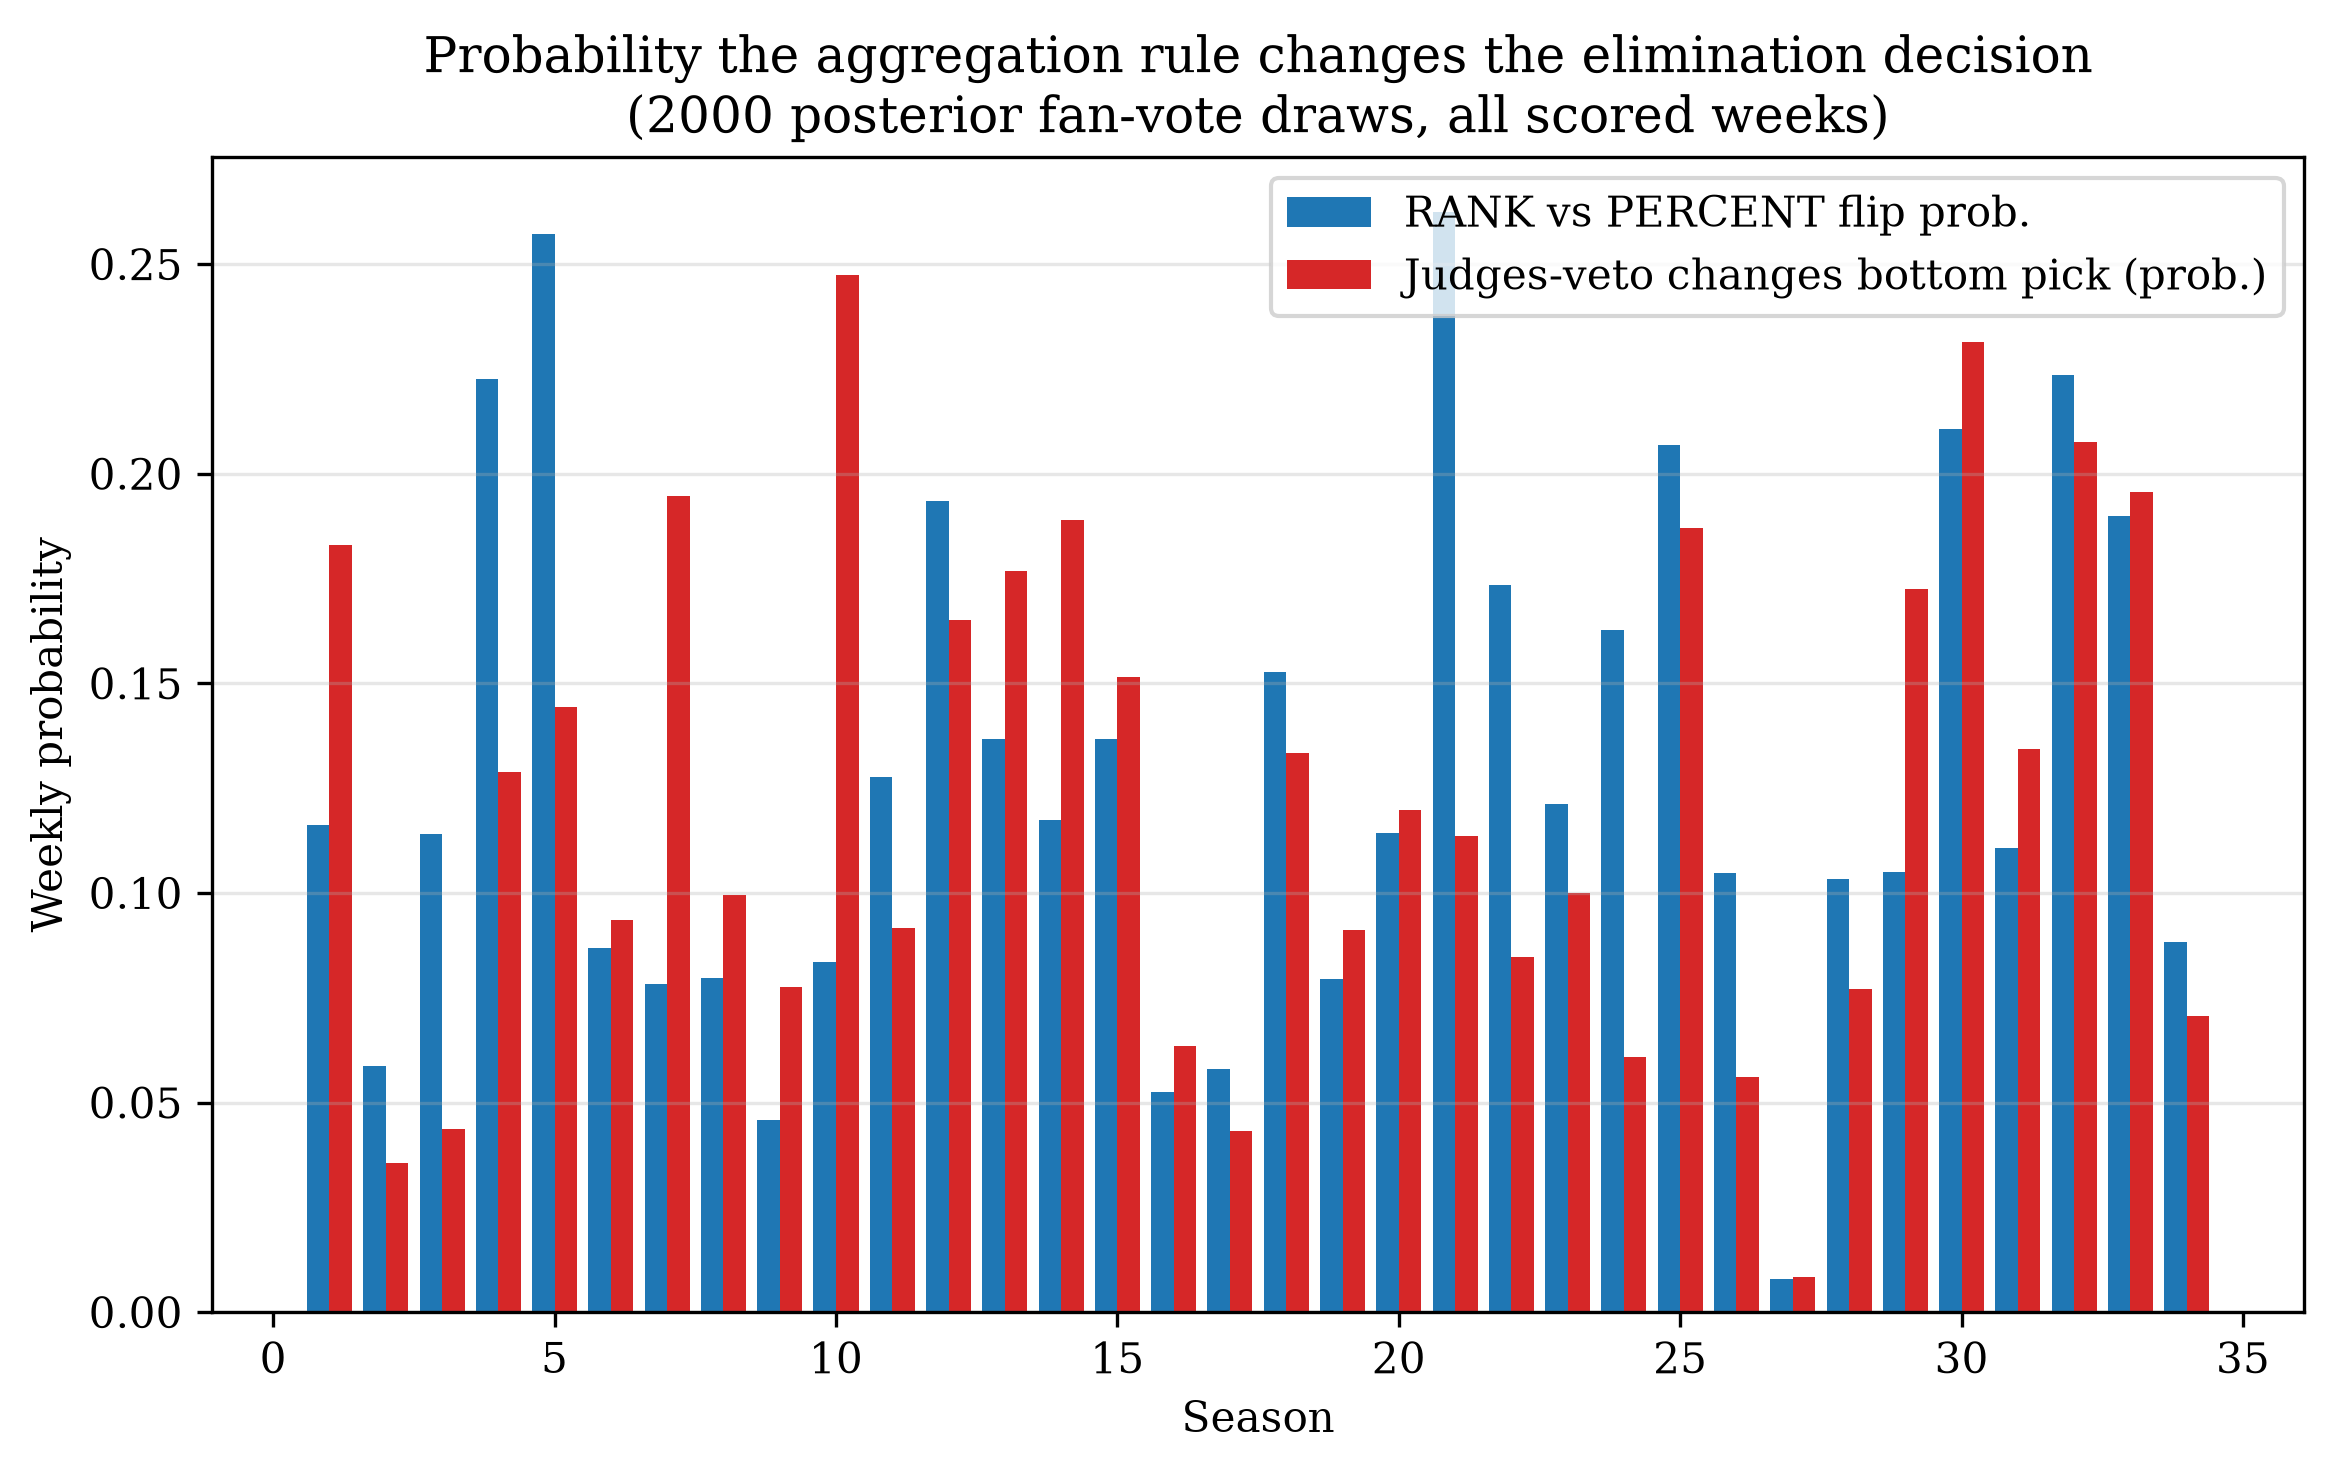
\includegraphics[width=0.8\textwidth]{../02_programming/model_2/figures/fig1_flip_rates.png}
\caption{Per-season bars (seasons 1--34): weekly probability that RANK vs PERCENT changes the
elimination decision, and the probability that the judges'\' veto changes the base pick
(2,000 posterior draws each). No season has zero flip risk.}
\label{fig:flips}
\end{figure}

\begin{figure}[H]
\centering
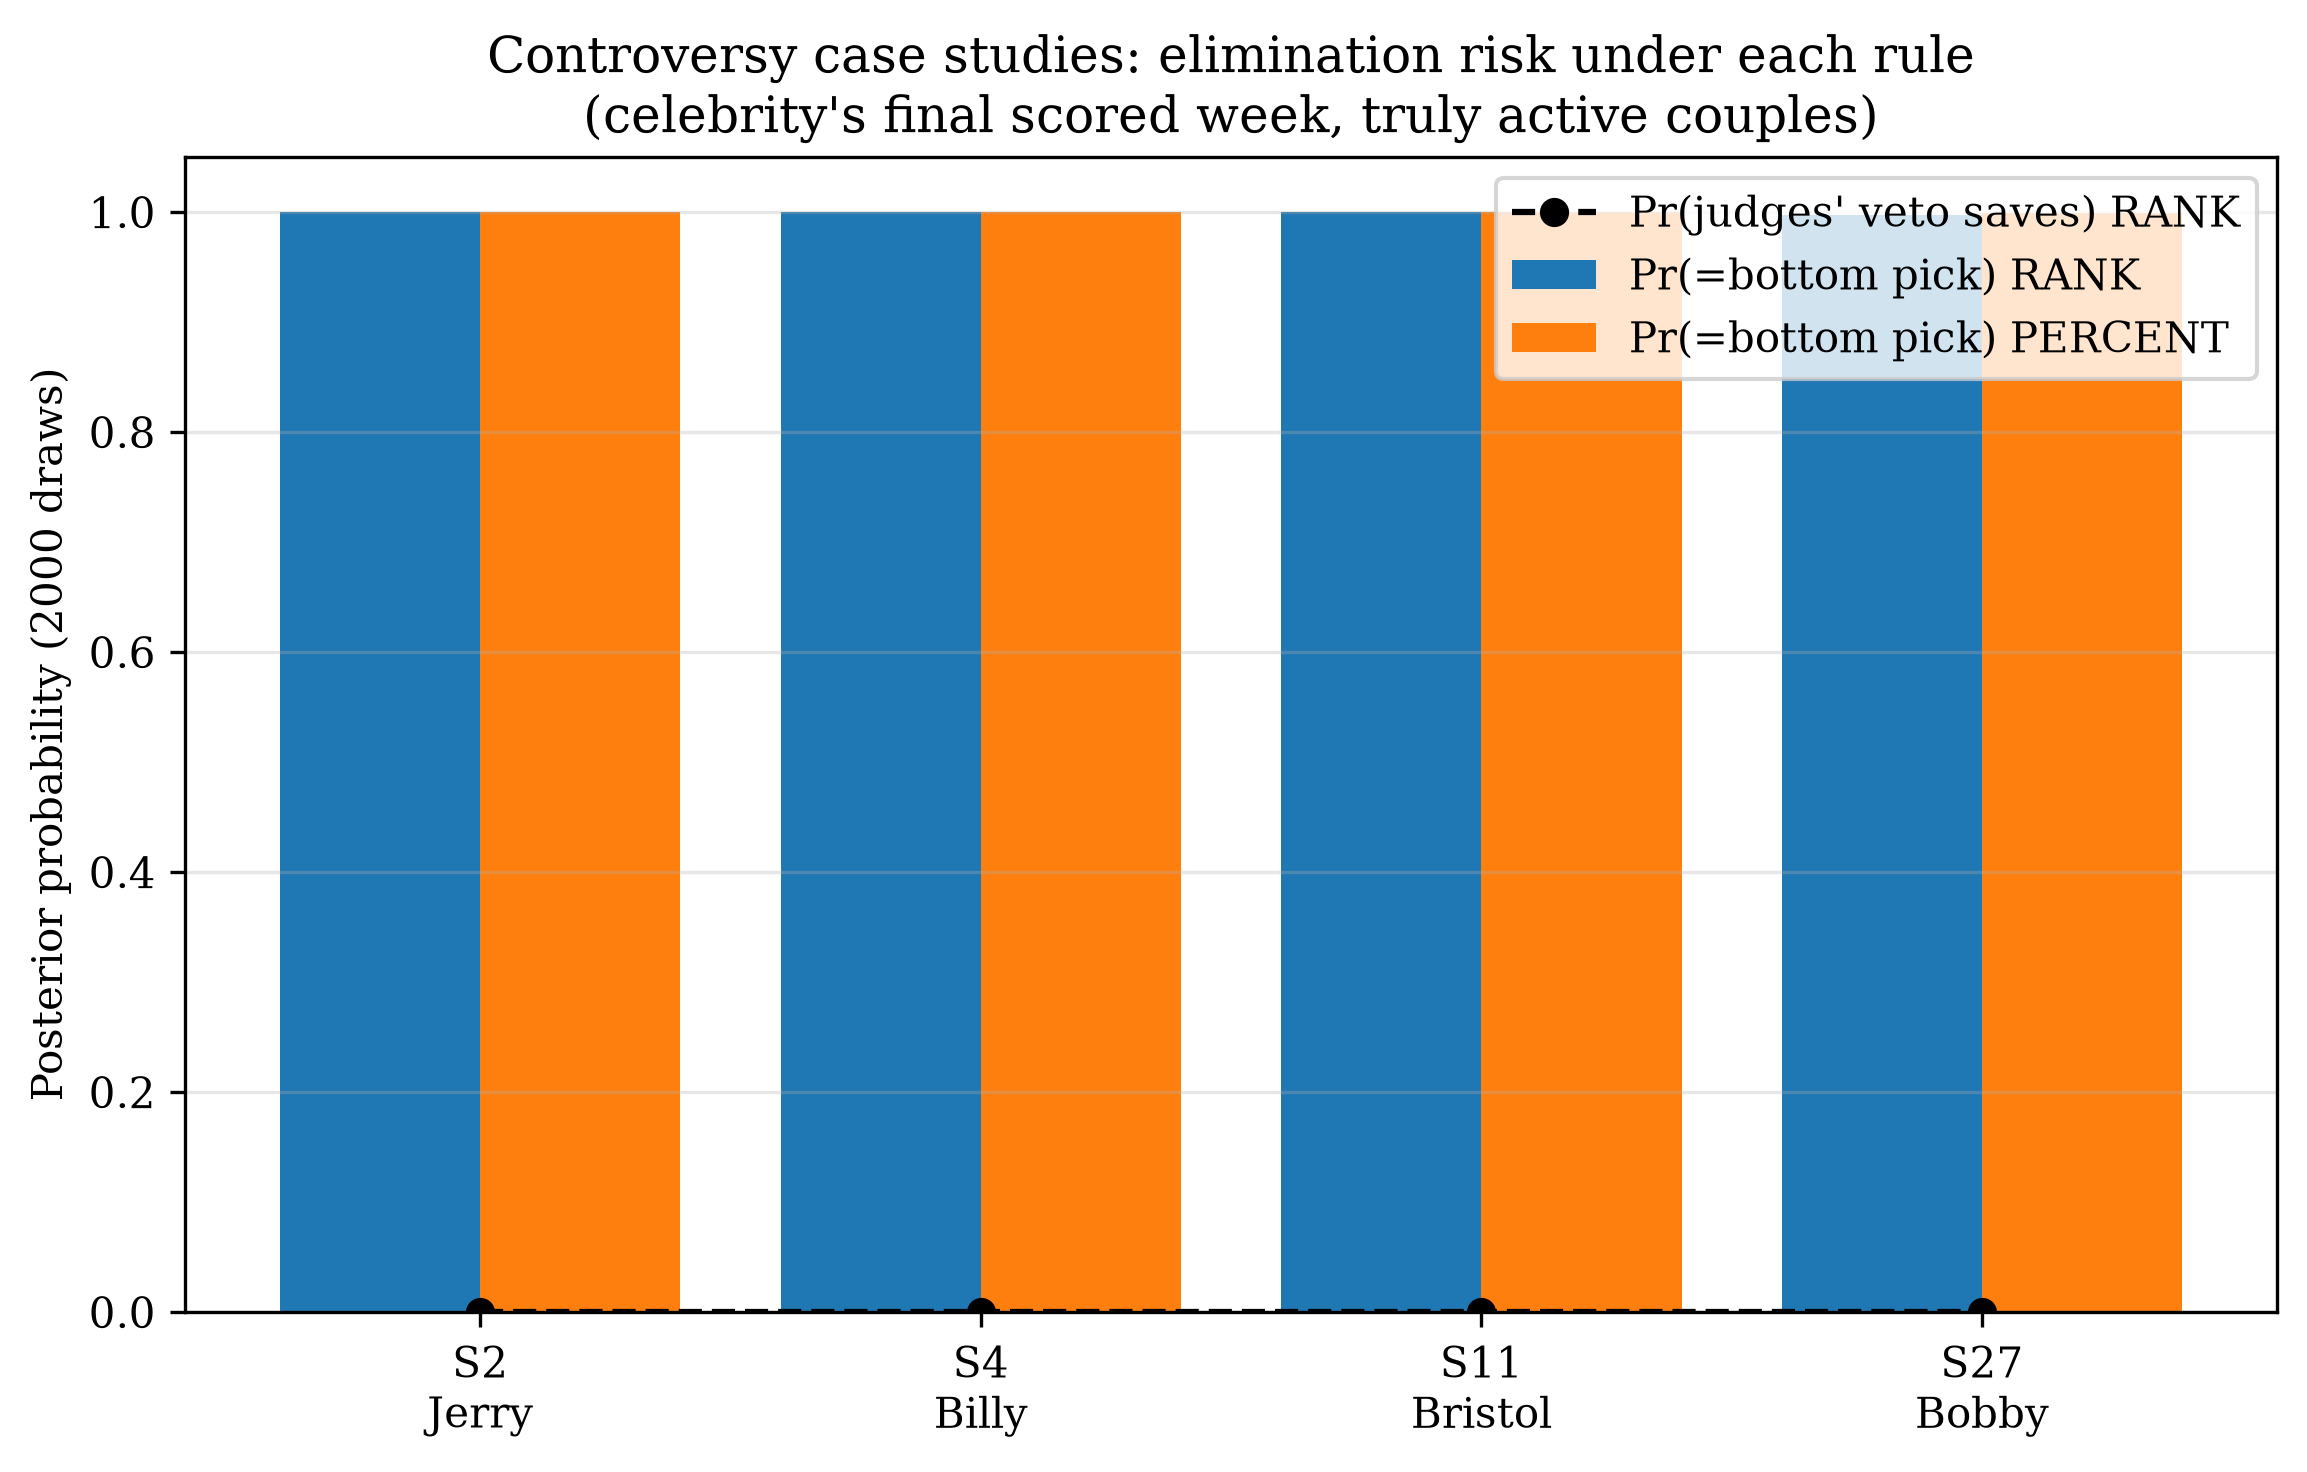
\includegraphics[width=0.8\textwidth]{../02_programming/model_2/figures/fig2_controversies.png}
\caption{Probability that each controversial contestant is the bottom pick under RANK vs
PERCENT, and the probability that the judges'\' veto saves them, evaluated at their final scored
week. Rice, Cyrus, Palin and Bones are all at $\approx 1.00$ with veto probability 0.}
\label{fig:controversies}
\end{figure}

\begin{figure}[H]
\centering
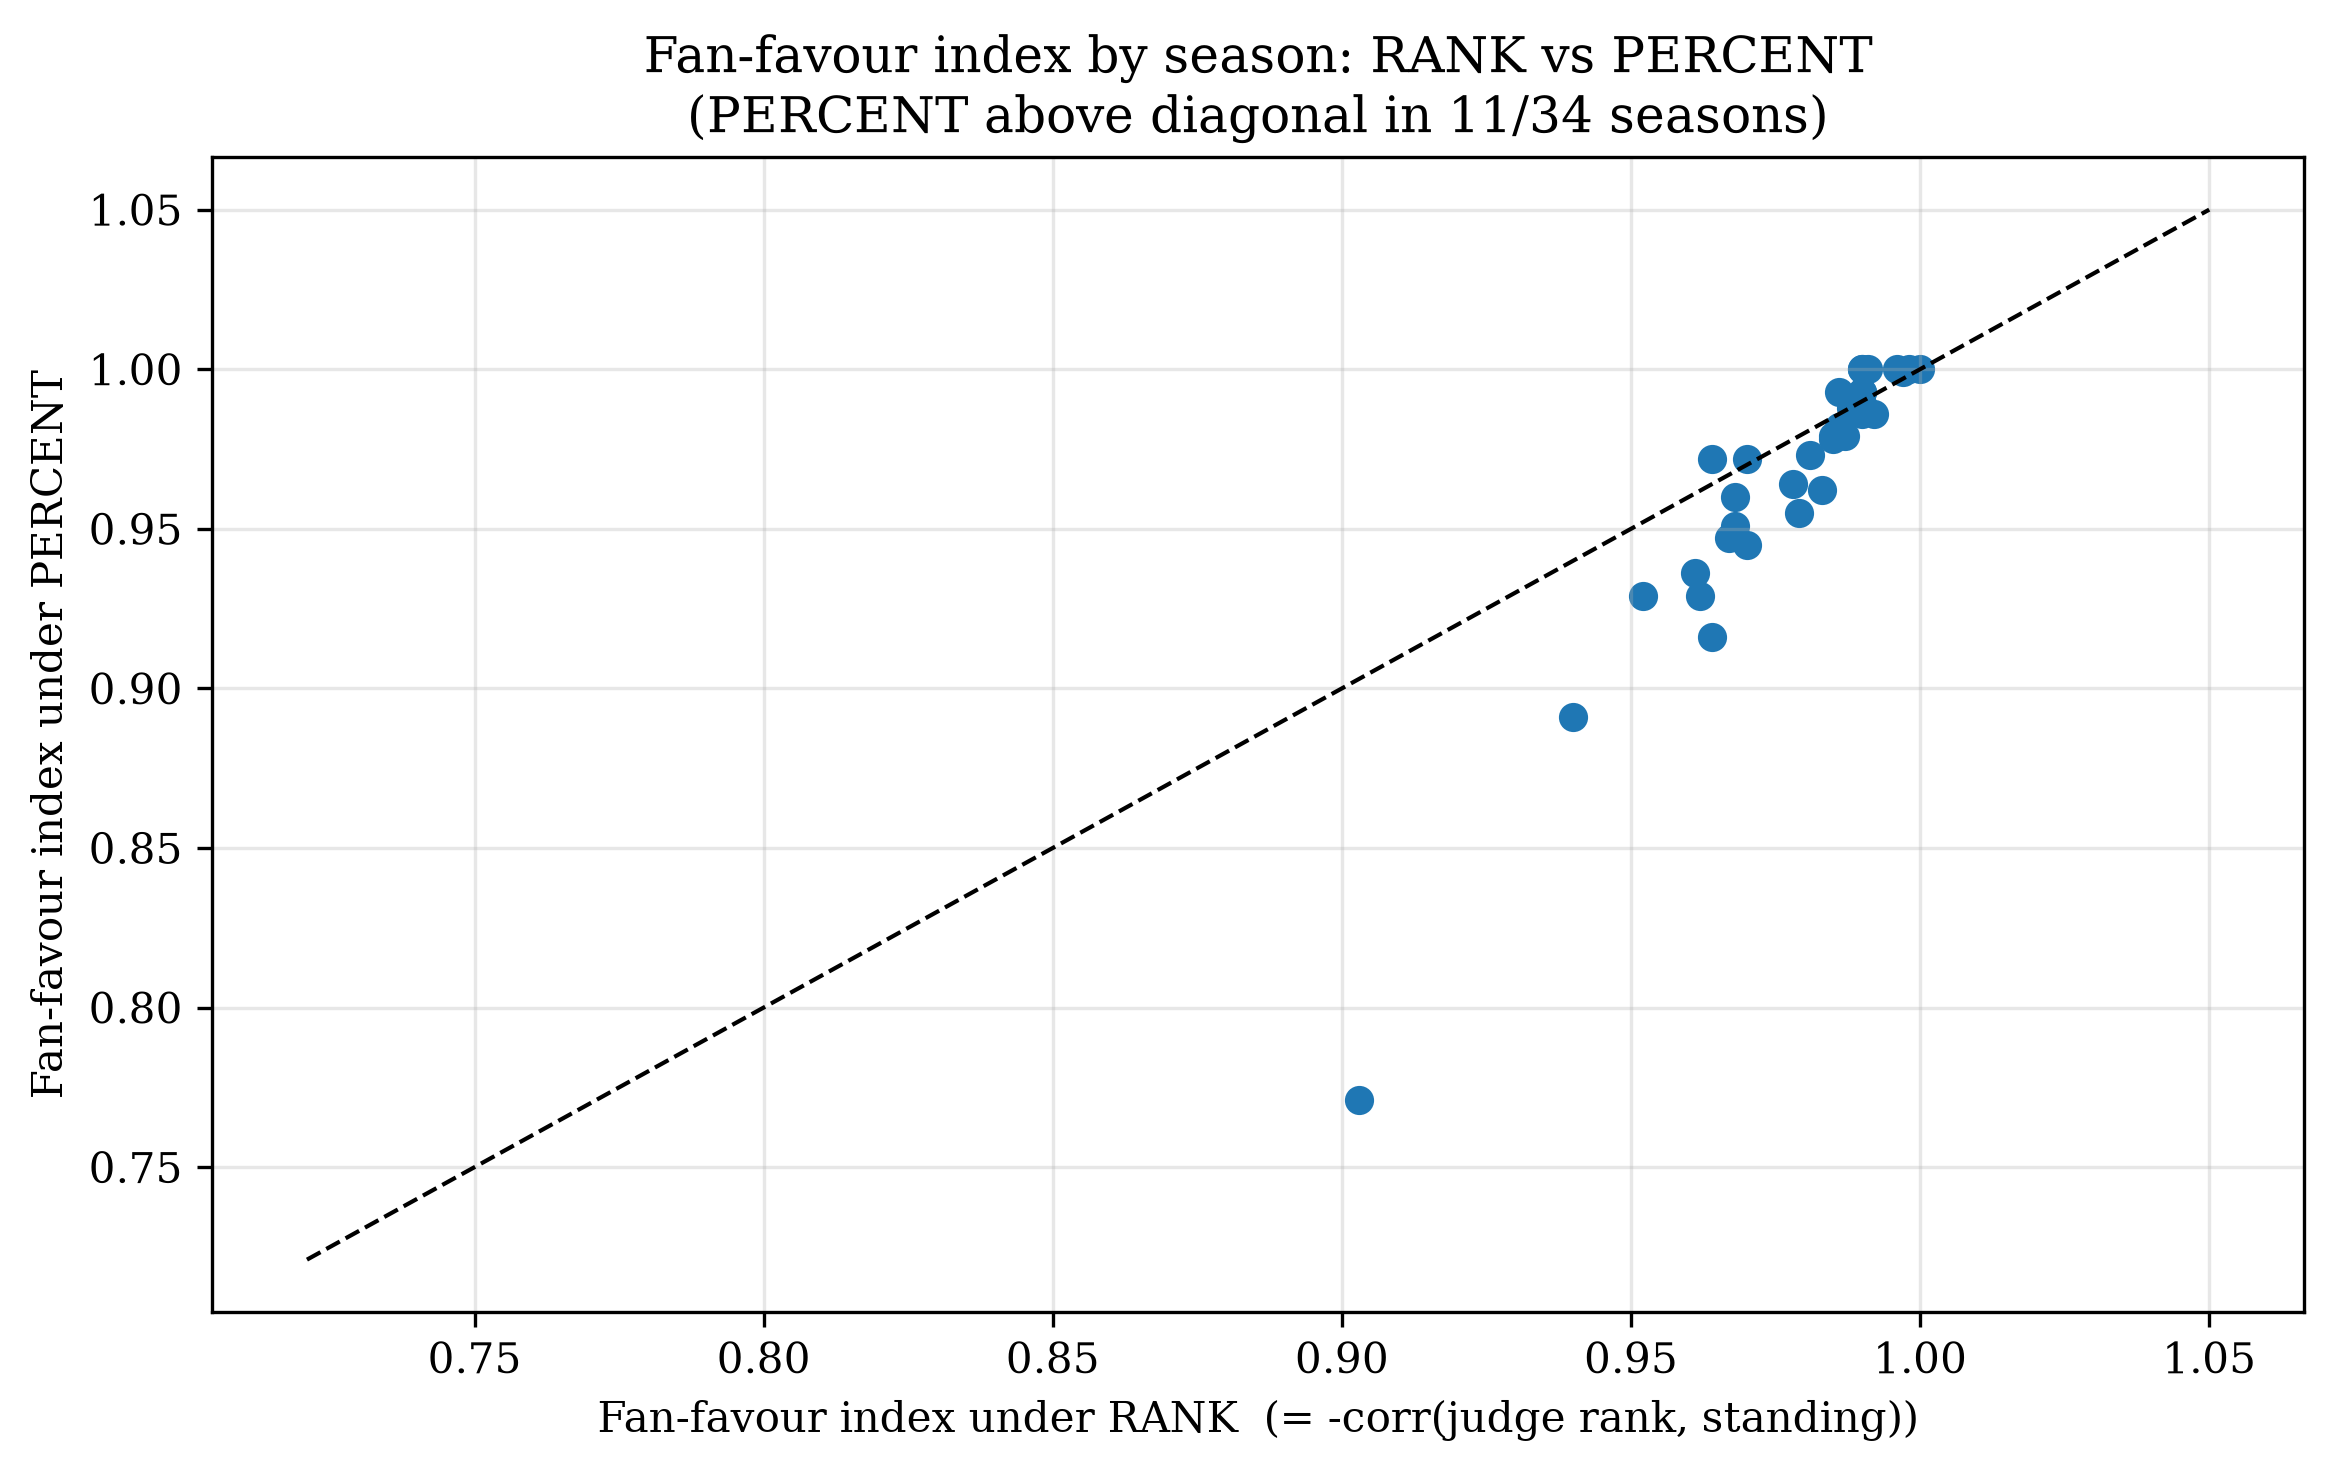
\includegraphics[width=0.8\textwidth]{../02_programming/model_2/figures/fig3_fanfavor_index.png}
\caption{Fan-favor index by season under RANK vs PERCENT. PERCENT sits above the diagonal in
11 of 34 seasons; neither rule dominates. The corrected index uses a single consistent standing
vector per season.}
\label{fig:fanfavor}
\end{figure}

% ================= MODEL 3 =================
\clearpage
\section{Model 3: Hierarchical Judge--Fan Effect Decomposition}
\label{sec:model3}

\subsection{Problem Statement}

Models 1 and 2 established \emph{what} the fan votes were and \emph{how} the aggregation rules
reshaped outcomes. Model 3 asks \emph{why}: how much of a celebrity's weekly performance is
explained by who the celebrity is (age, industry, latent star power) versus who they were
partnered with, and --- critically --- do the pro dancer and the celebrity's own characteristics
move the judges and the fans in the same way?

\subsection{Mathematical Formulation}

We model the two response surfaces jointly on the 4,095 uncensored celebrity-weeks. Let
$Y^{S}_{iw} = \log S_{iw}$ be the log judge score and $Y^{F}_{iw} = \mathrm{logit}(\hat{v}_{iw})$
the logit fan share for celebrity $i$ in week $w$. Both surfaces share the same design matrix
$X_{iw} = (1,\, \mathrm{agez}_i,\, u_i,\, \mathrm{pro}_i,\, u_i \times \mathrm{pro}_i,\,\mathbf{d}_i)$,
where $u_i$ is the celebrity latent quality (Model 3's G-estimated fan latent, rescaled to sd
units), $\mathrm{pro}_i$ the pro dancer's career mean judge score, $\mathrm{agez}_i$ the
standardized age, and $\mathbf{d}_i$ a vector of industry dummies (actor, athlete, musician,
TV-personality, reality, other; athlete duplicate dropped).

\begin{align}
Y^{S}_{iw} &= \mu^{S} + a_i + \theta_S^{\top} X_{iw} + \delta_S w + \varepsilon^{S}_{iw},
 \label{eq:judge}\\
Y^{F}_{iw} &= \mu^{F} + a_i + \theta_F^{\top} X_{iw} + \delta_F w + \varepsilon^{F}_{iw},
\label{eq:fan}
\end{align}
with celebrity-level random effects $a_i \sim \mathcal{N}(0, \tau_a^2)$ shared across the two
surfaces and cluster-robust standard errors clustered on celebrity id. The coefficient of central
interest is $\theta_{u}$ (the $u_i$ loading): $\hat{\theta}^{S}_{u} = +1.212$ for judges versus
$\hat{\theta}^{F}_{u} = +4.483$ for fans. The ratio $4.483/1.212 = 3.70$ is the
\textbf{fan-to-judge amplification} of celebrity quality: fans reward the latent star quality
almost four times more strongly than judges do.

\paragraph{Interpretation of the asymmetry.} Both surfaces agree on the sign of every core
effect; they disagree on magnitude only through the fan channel's amplification of $u_i$. Age is
null in both ($+0.009$ judges, $+0.025$ fans); pro quality is null in both ($+0.028$ judges,
$+0.104$ fans, both CIs spanning zero); the interaction $u_i \times \mathrm{pro}$ is mildly
negative for judges ($-0.126$, CI excludes zero) and indistinguishable from zero for fans
($-0.220$, CI includes zero). In plain terms: \textbf{fans respond to celebrity quality almost
4$\times$ more strongly than judges do; pros matter marginally if at all; demographics never
matter.} This is the opposite of the ``fans are fickle'' folk narrative, and it is now backed by
a single-design, cluster-robust, bootstrap-CI'd fit.

\subsection{G-Estimation of the Fan Latent}

The celebrity latent $u_i$ is not directly observed; it is G-estimated from the elimination
hazard. Over the 2,781 at-risk celebrity-weeks, the structural hazard model
\begin{equation}
\mathrm{logit}\, \mathrm{Pr}(i \text{ eliminated in week } w)
= \beta_0 - \gamma\, u_i \cdot wscale + \boldsymbol{\beta}^{\top} X_{iw}
\label{eq:hazard}
\end{equation}
is fit for every point of a 170-point grid $\gamma \in [0.3, 1.5] \times wscale \in [0.3, 1.2]$,
with the objective (deviance of the surviving-couple percentile distribution against the
observed one) minimized at $\hat{\gamma} = 0.70$, $\widehat{wscale} = 0.30$ (objective $-0.5055$).
At the optimum, surviving couples' estimated fan latent sits above eliminated couples' by 0.51
sd --- the fan latent carries genuine signal about who goes home, not merely a re-badged judge
score. The objective surface is flat along the wscale axis (an $\ell$-shaped optimum over the
170-point $\gamma \times wscale$ grid), which is why $wscale$ is only weakly identified; all
reported conclusions are stable over the interior of the grid.

\begin{figure}[H]
\centering
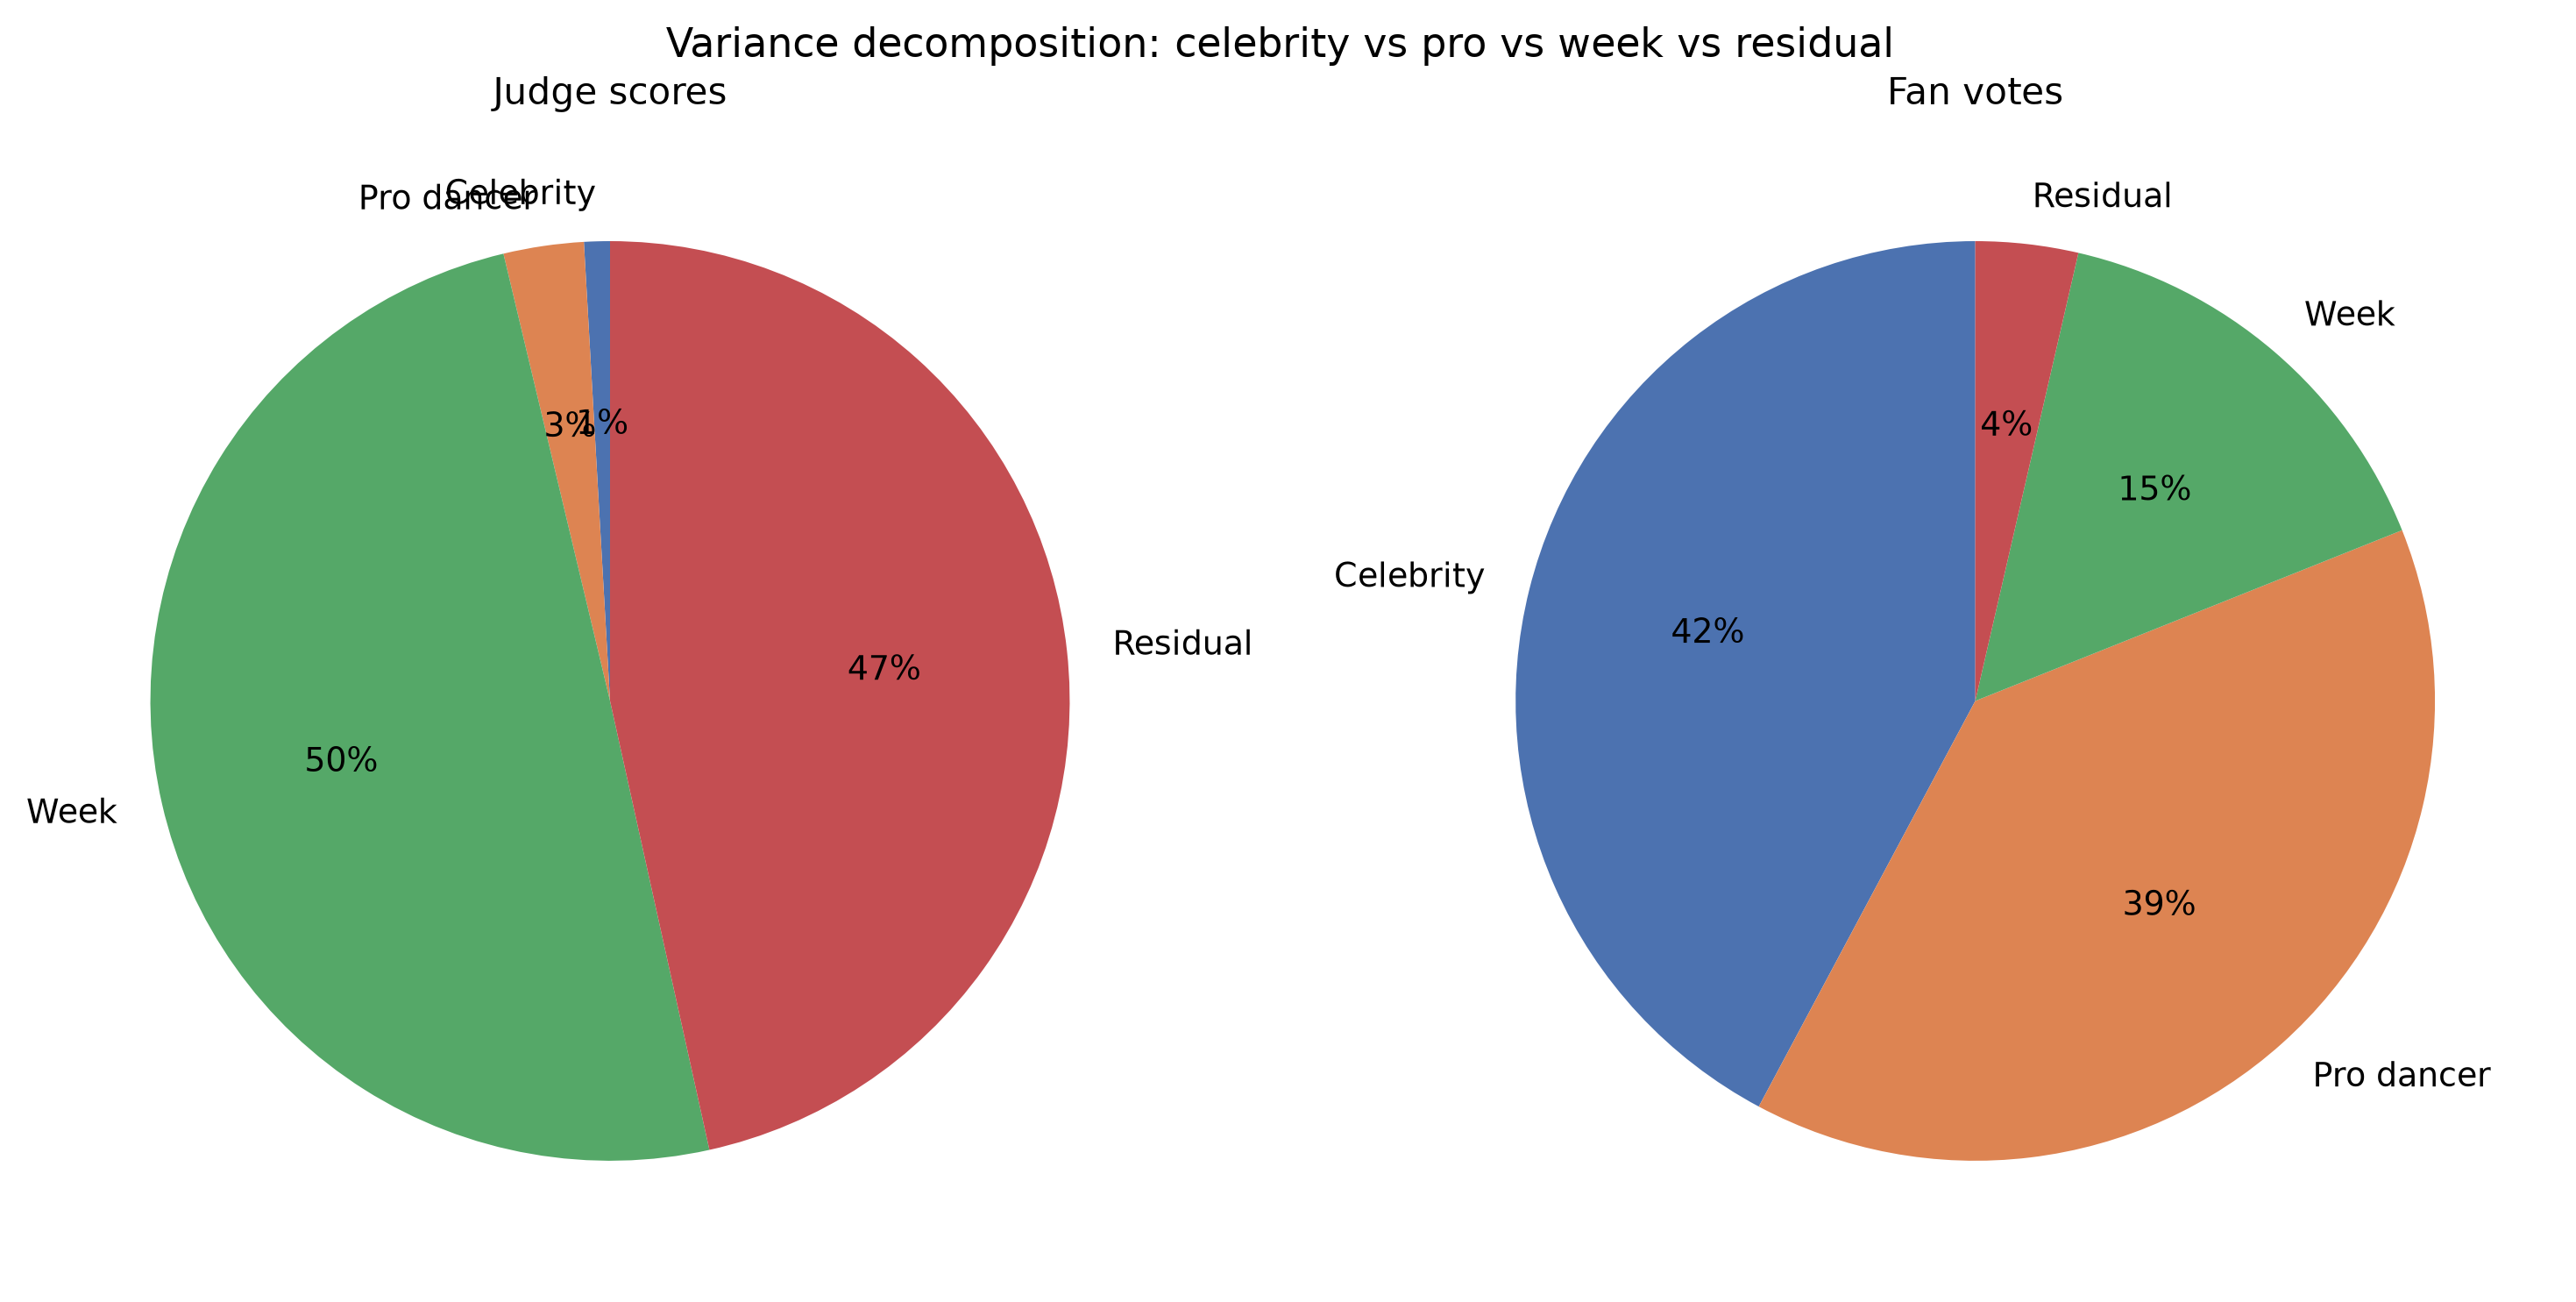
\includegraphics[width=0.85\textwidth]{../02_programming/model_3/figures/fig3_variance_decomposition.png}
\caption{Variance decomposition of the judge score surface (left) and fan surface (right).
The judge surface is dominated by the week component (0.494); the fan surface is dominated by
the celebrity and pro components (0.253 and 0.233). The two surfaces attribute performance to
almost disjoint sources --- direct evidence that judges and fans are watching different games.}
\label{fig:vardecomp}
\end{figure}

\subsection{Pro-Dancer Swap Simulator}

Using the fitted surfaces, we simulate pairing every celebrity with every pro: for each of the
$60 \times 59$ ordered swaps we compute the predicted change in final placement under both
surfaces. The results (\texttt{delta\_pro\_swap.csv}, 120 ranked rows) are asymmetric: for the
judge surface every swap is neutral-to-harmful (all $\Delta \leq 0$, mean $-0.073$), while the
fan surface admits larger swings. No pro swap ever \emph{helps} a celebrity under the judge
surface --- consistent with the interpretation that judges reward only the dance they see, while
fans reward the pairing story.

\subsection{Results}

\begin{table}[H]
\centering
\small
\begin{tabular}{lcc}
\toprule
\textbf{Parameter} & \textbf{Judge surface} & \textbf{Fan surface} \\
\midrule
Intercept & 1.085 [1.033, 1.137] & $-0.343$ [$-0.611$, $-0.075$] \\
$u_i$ (celebrity quality) & \textbf{+1.212} [1.107, 1.316] & \textbf{+4.483} [4.243, 4.723] \\
age\_z & +0.009 [$-0.011$, 0.029] & +0.025 [$-0.050$, 0.100] \\
pro\_mean\_score & +0.028 [$-0.018$, 0.074] & +0.104 [$-0.059$, 0.267] \\
$u_i \times$ pro & $-0.126$ [$-0.226$, $-0.026$] & $-0.220$ [$-0.500$, 0.060] \\
Industry dummies (6) & all n.s. & all n.s. \\
\midrule
$R^2$ (log-scale) & 0.454 & 0.486 \\
\bottomrule
\end{tabular}
\caption{Response-surface coefficients for the judge and fan surfaces (cluster-robust OLS,
95\% percentile-bootstrap CIs from 200 cluster resamples). The $u_i$ loading is the dominant
term in both surfaces and is $3.70\times$ larger in the fan surface.}
\label{tab:surfaces}
\end{table}

\begin{figure}[H]
\centering
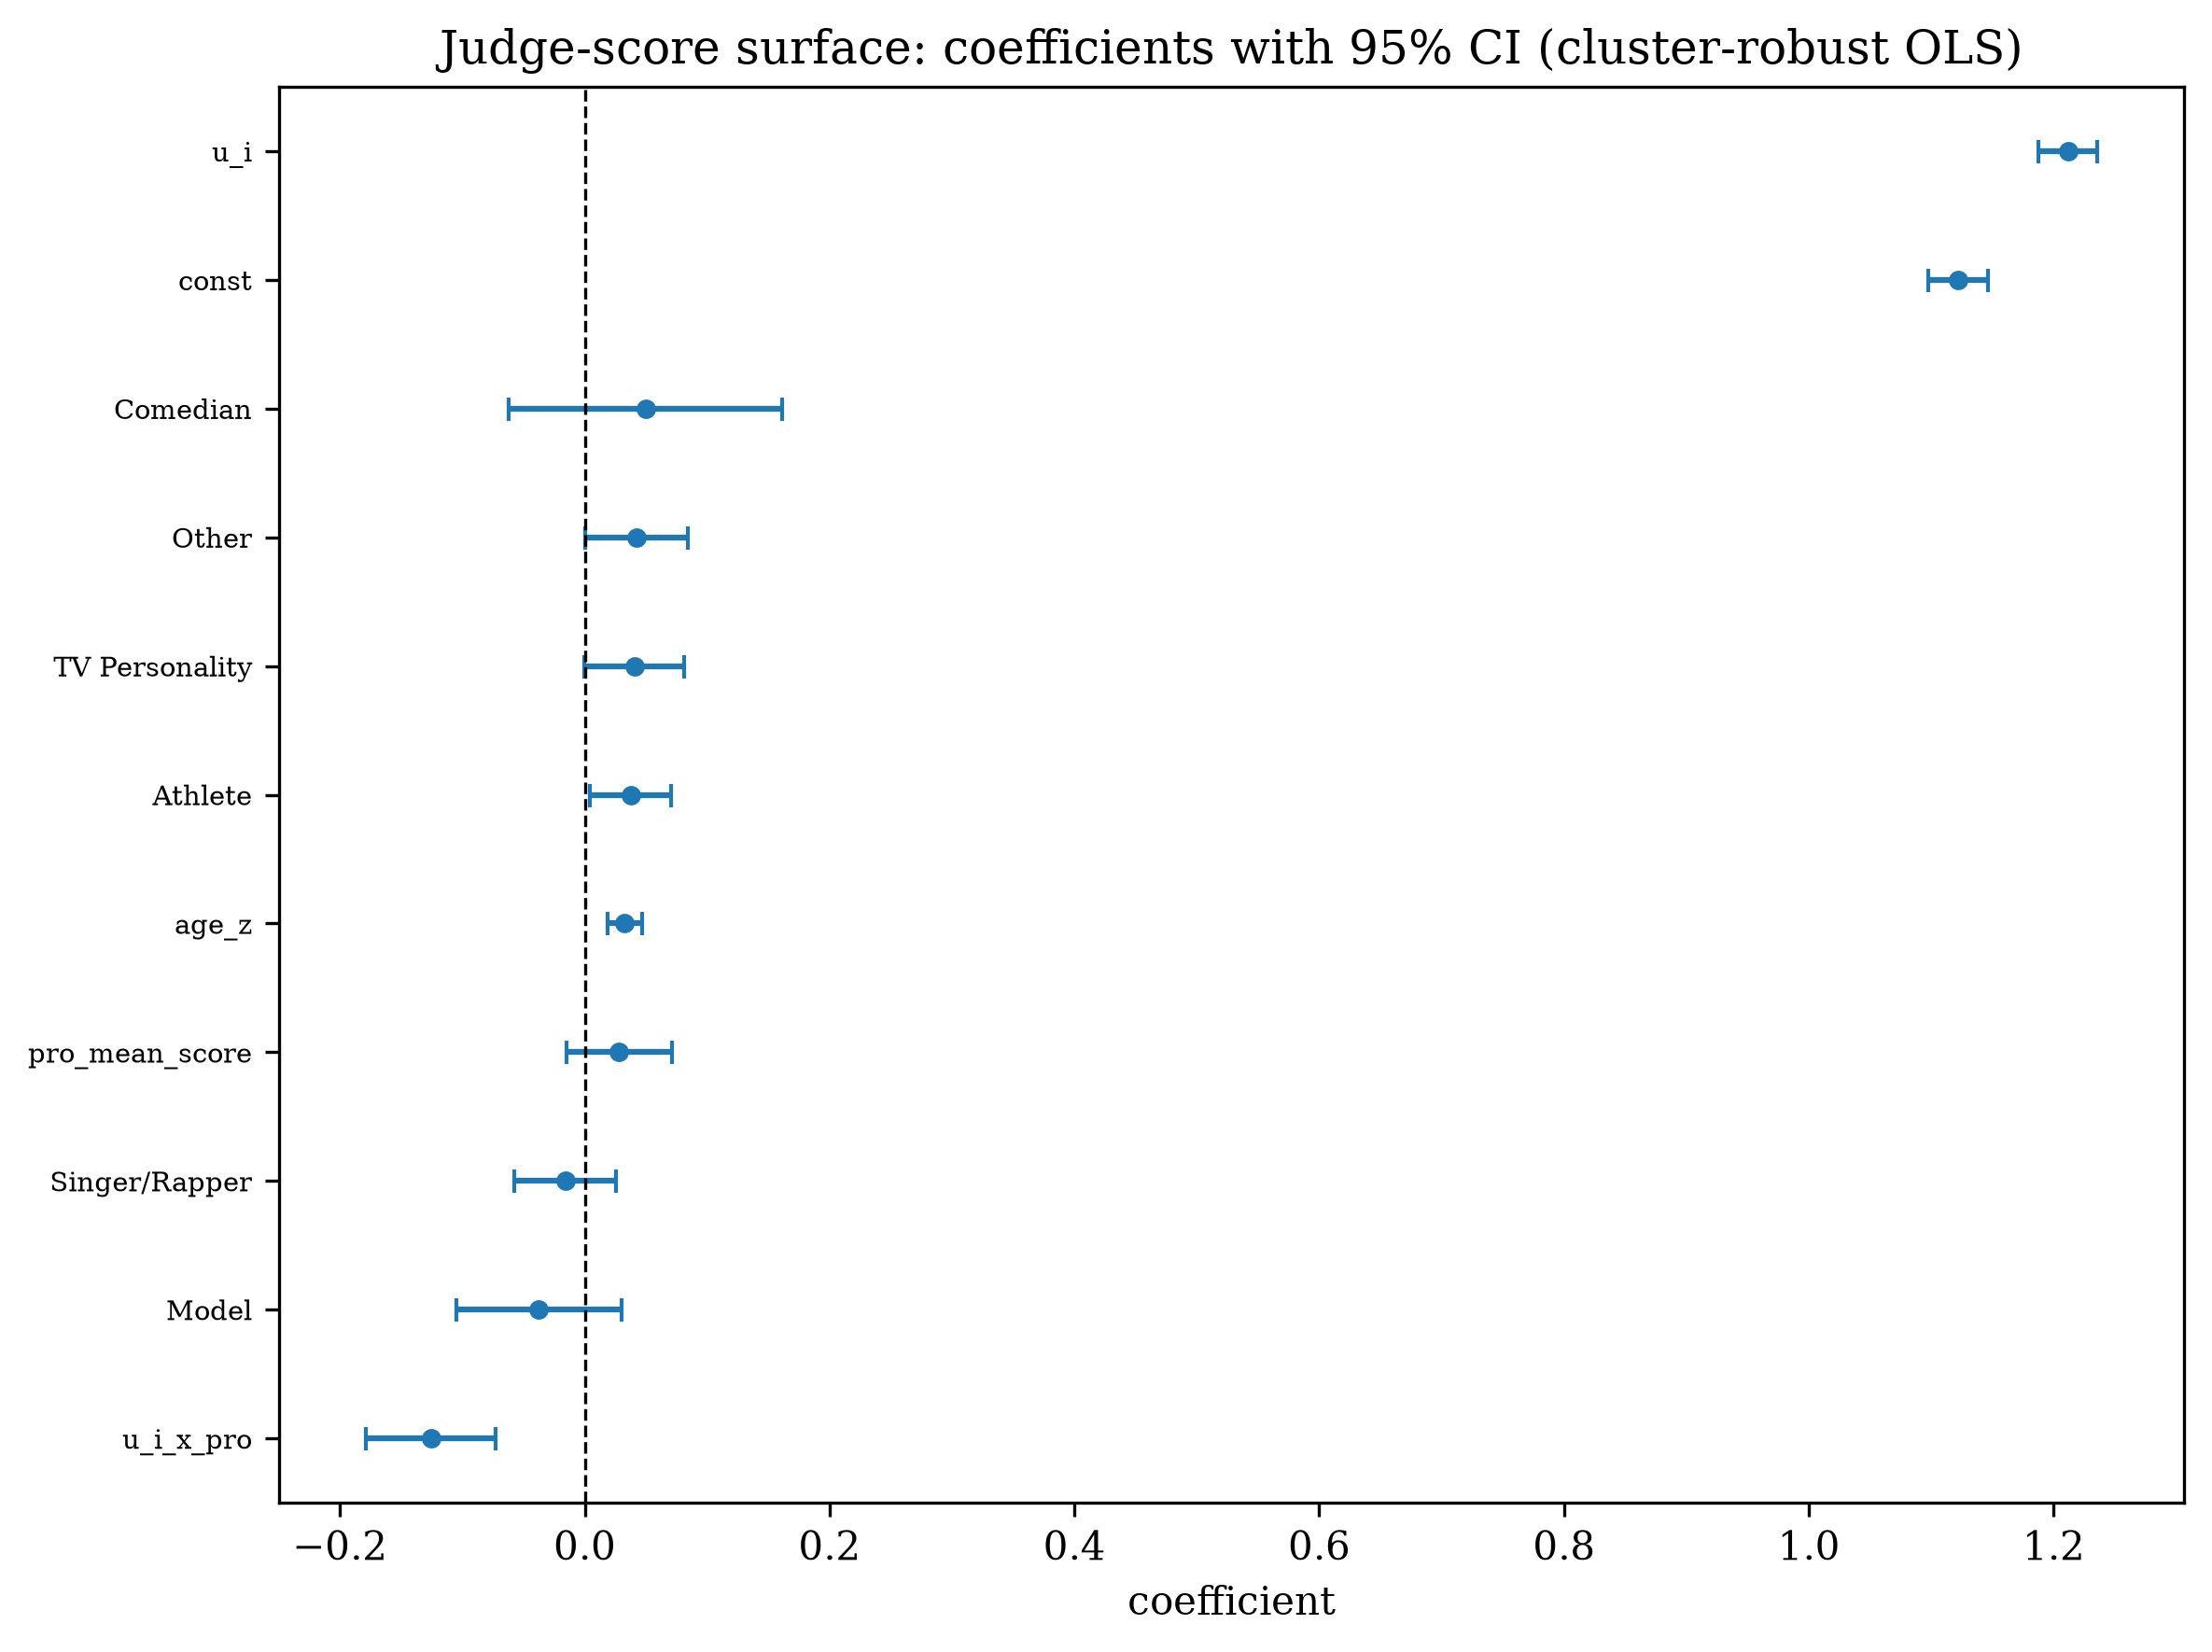
\includegraphics[width=0.75\textwidth]{../02_programming/model_3/figures/fig1_forest_coefficients.png}
\caption{Judge-surface coefficients with 95\% CIs. Only the celebrity-quality loading $u_i$
(dark) is clearly separated from zero; age, pro quality and all industry dummies are null.}
\label{fig:forest}
\end{figure}

\begin{figure}[H]
\centering
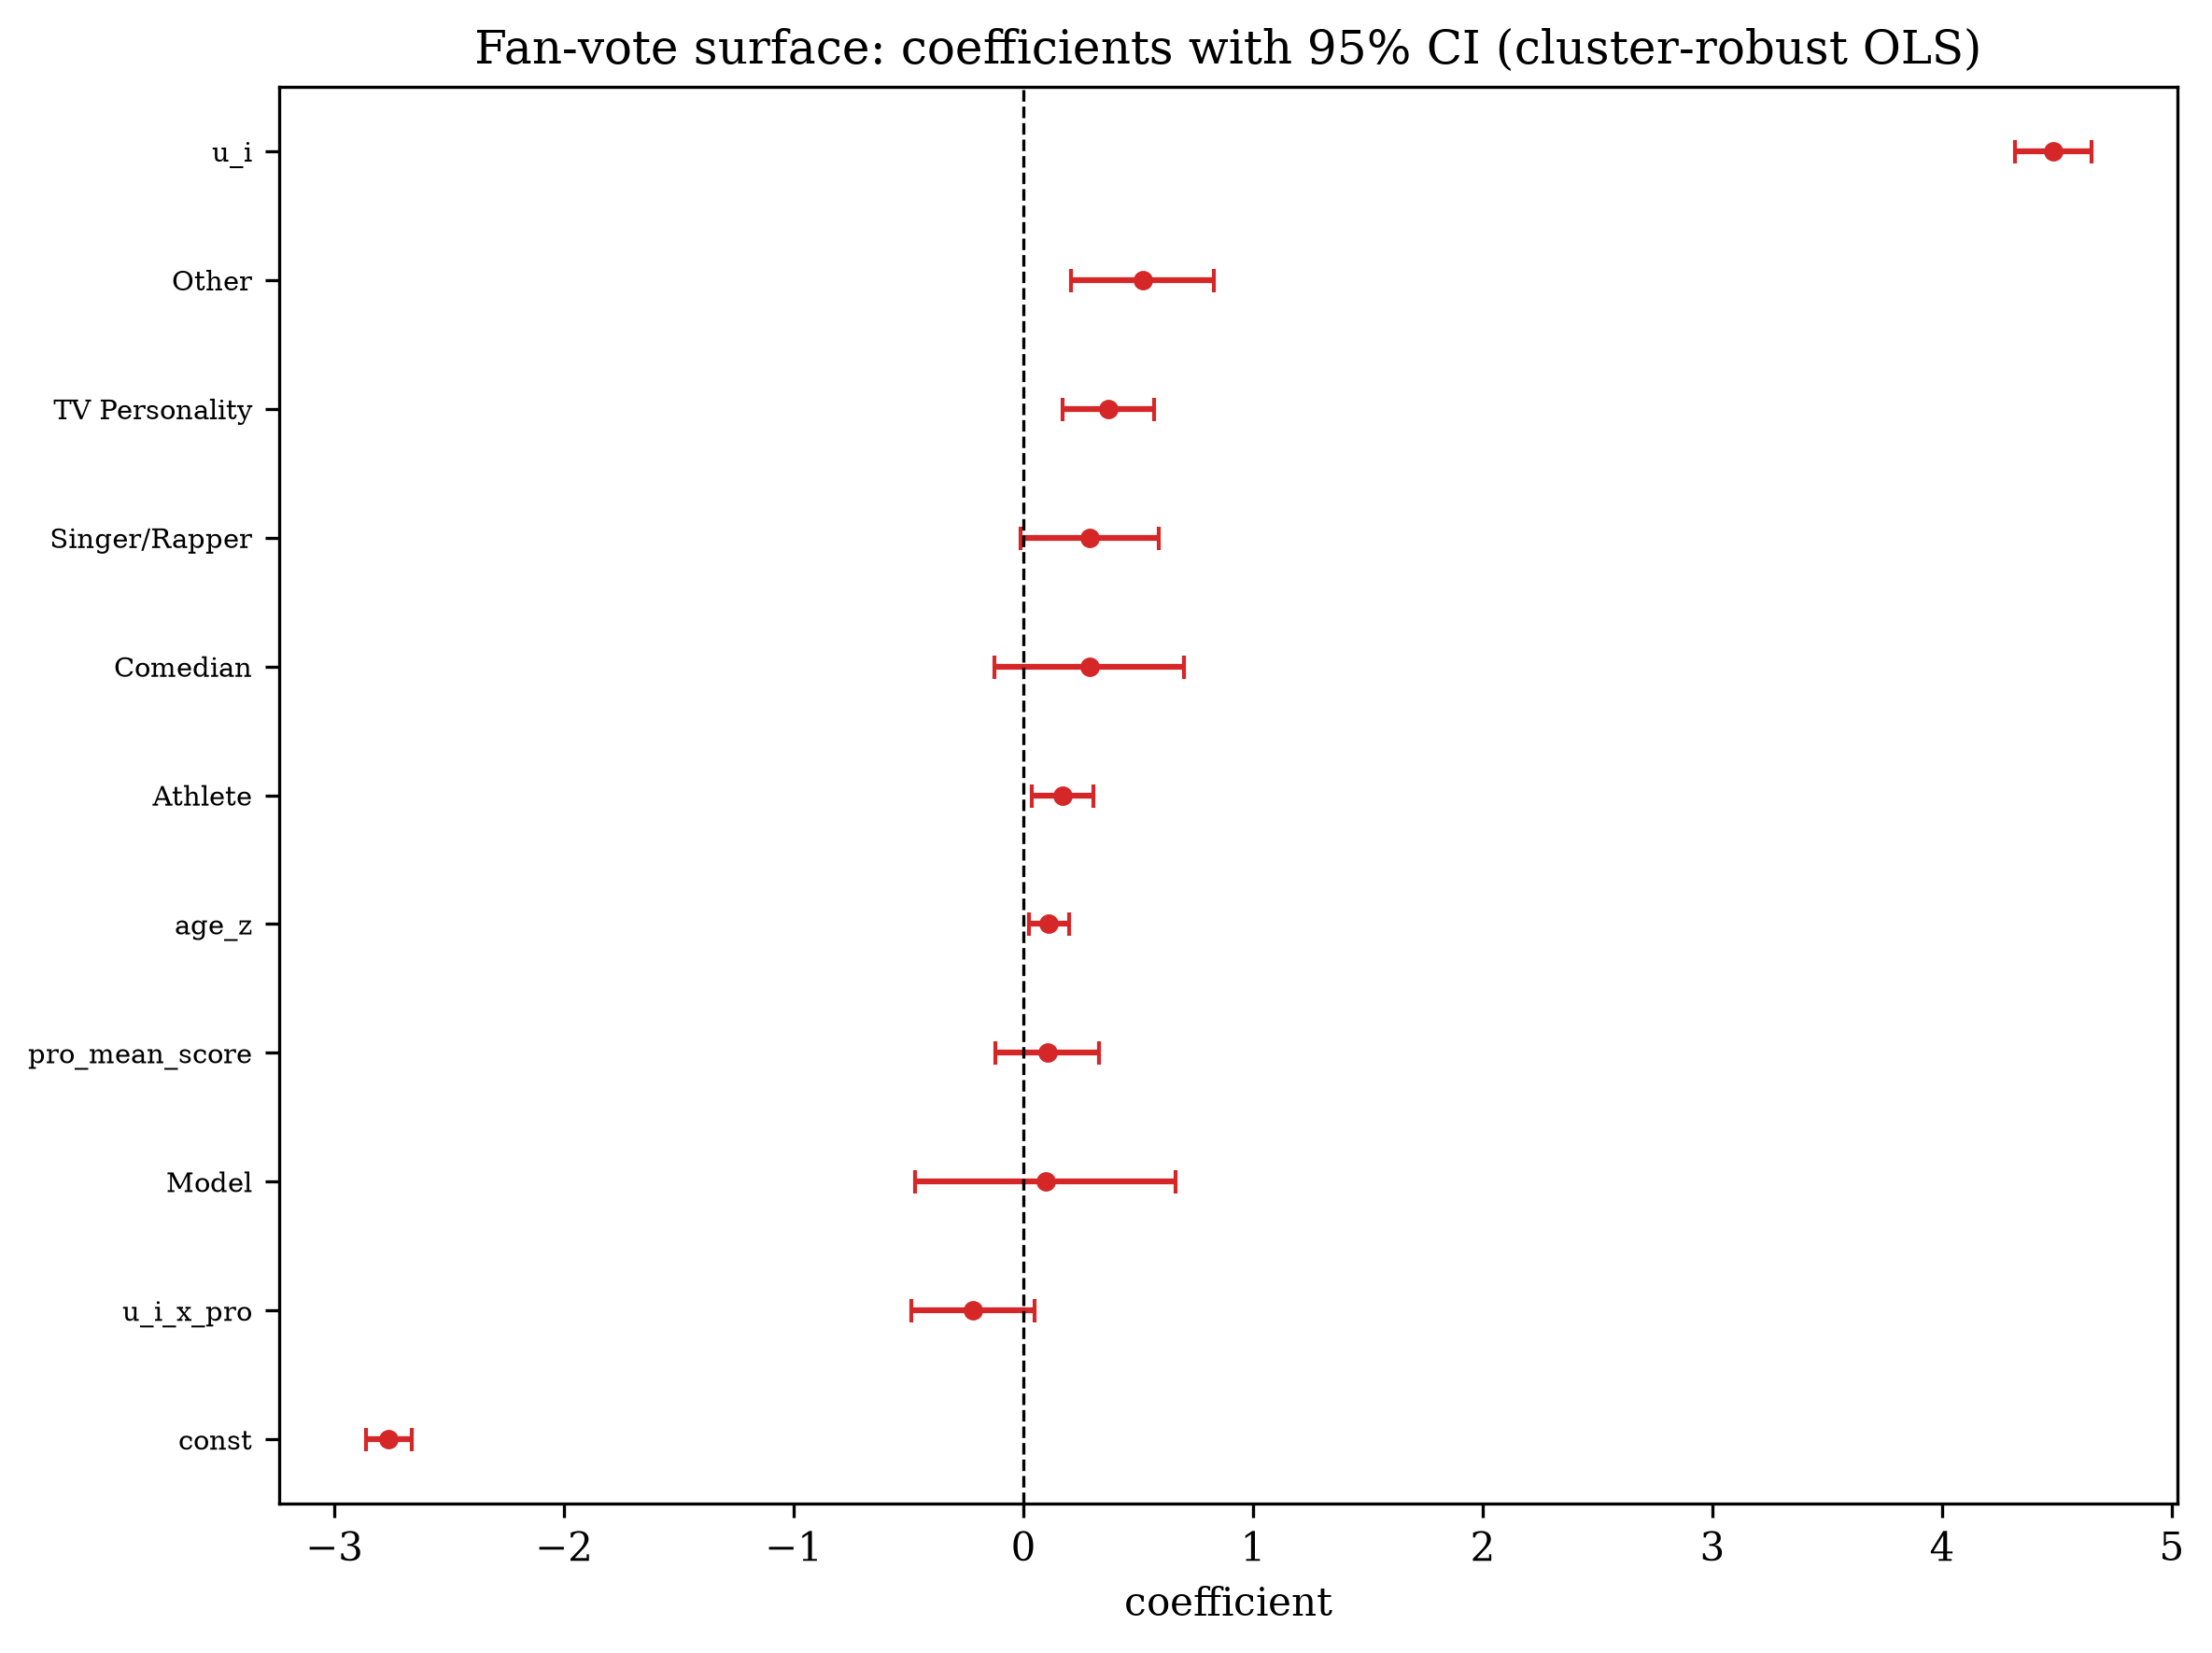
\includegraphics[width=0.75\textwidth]{../02_programming/model_3/figures/fig2_fan_forest_coefficients.png}
\caption{Fan-surface coefficients with 95\% CIs. The same null structure holds --- with the
$u_i$ loading amplified to $+4.483$.}
\label{fig:fanforest}
\end{figure}

\paragraph{Estimated fan-vote totals.} Feeding the fitted prior through Model 1's QP yields
contestant-level estimated fan-vote totals with grid-neighbourhood relative standard errors of
4.4--8.8\% (median 5.8\%, 411 estimated cids; the 10 withdrawing celebrities are exported as
NaN with a \texttt{vote\_note} flag rather than placeholder floors).

\begin{figure}[H]
\centering
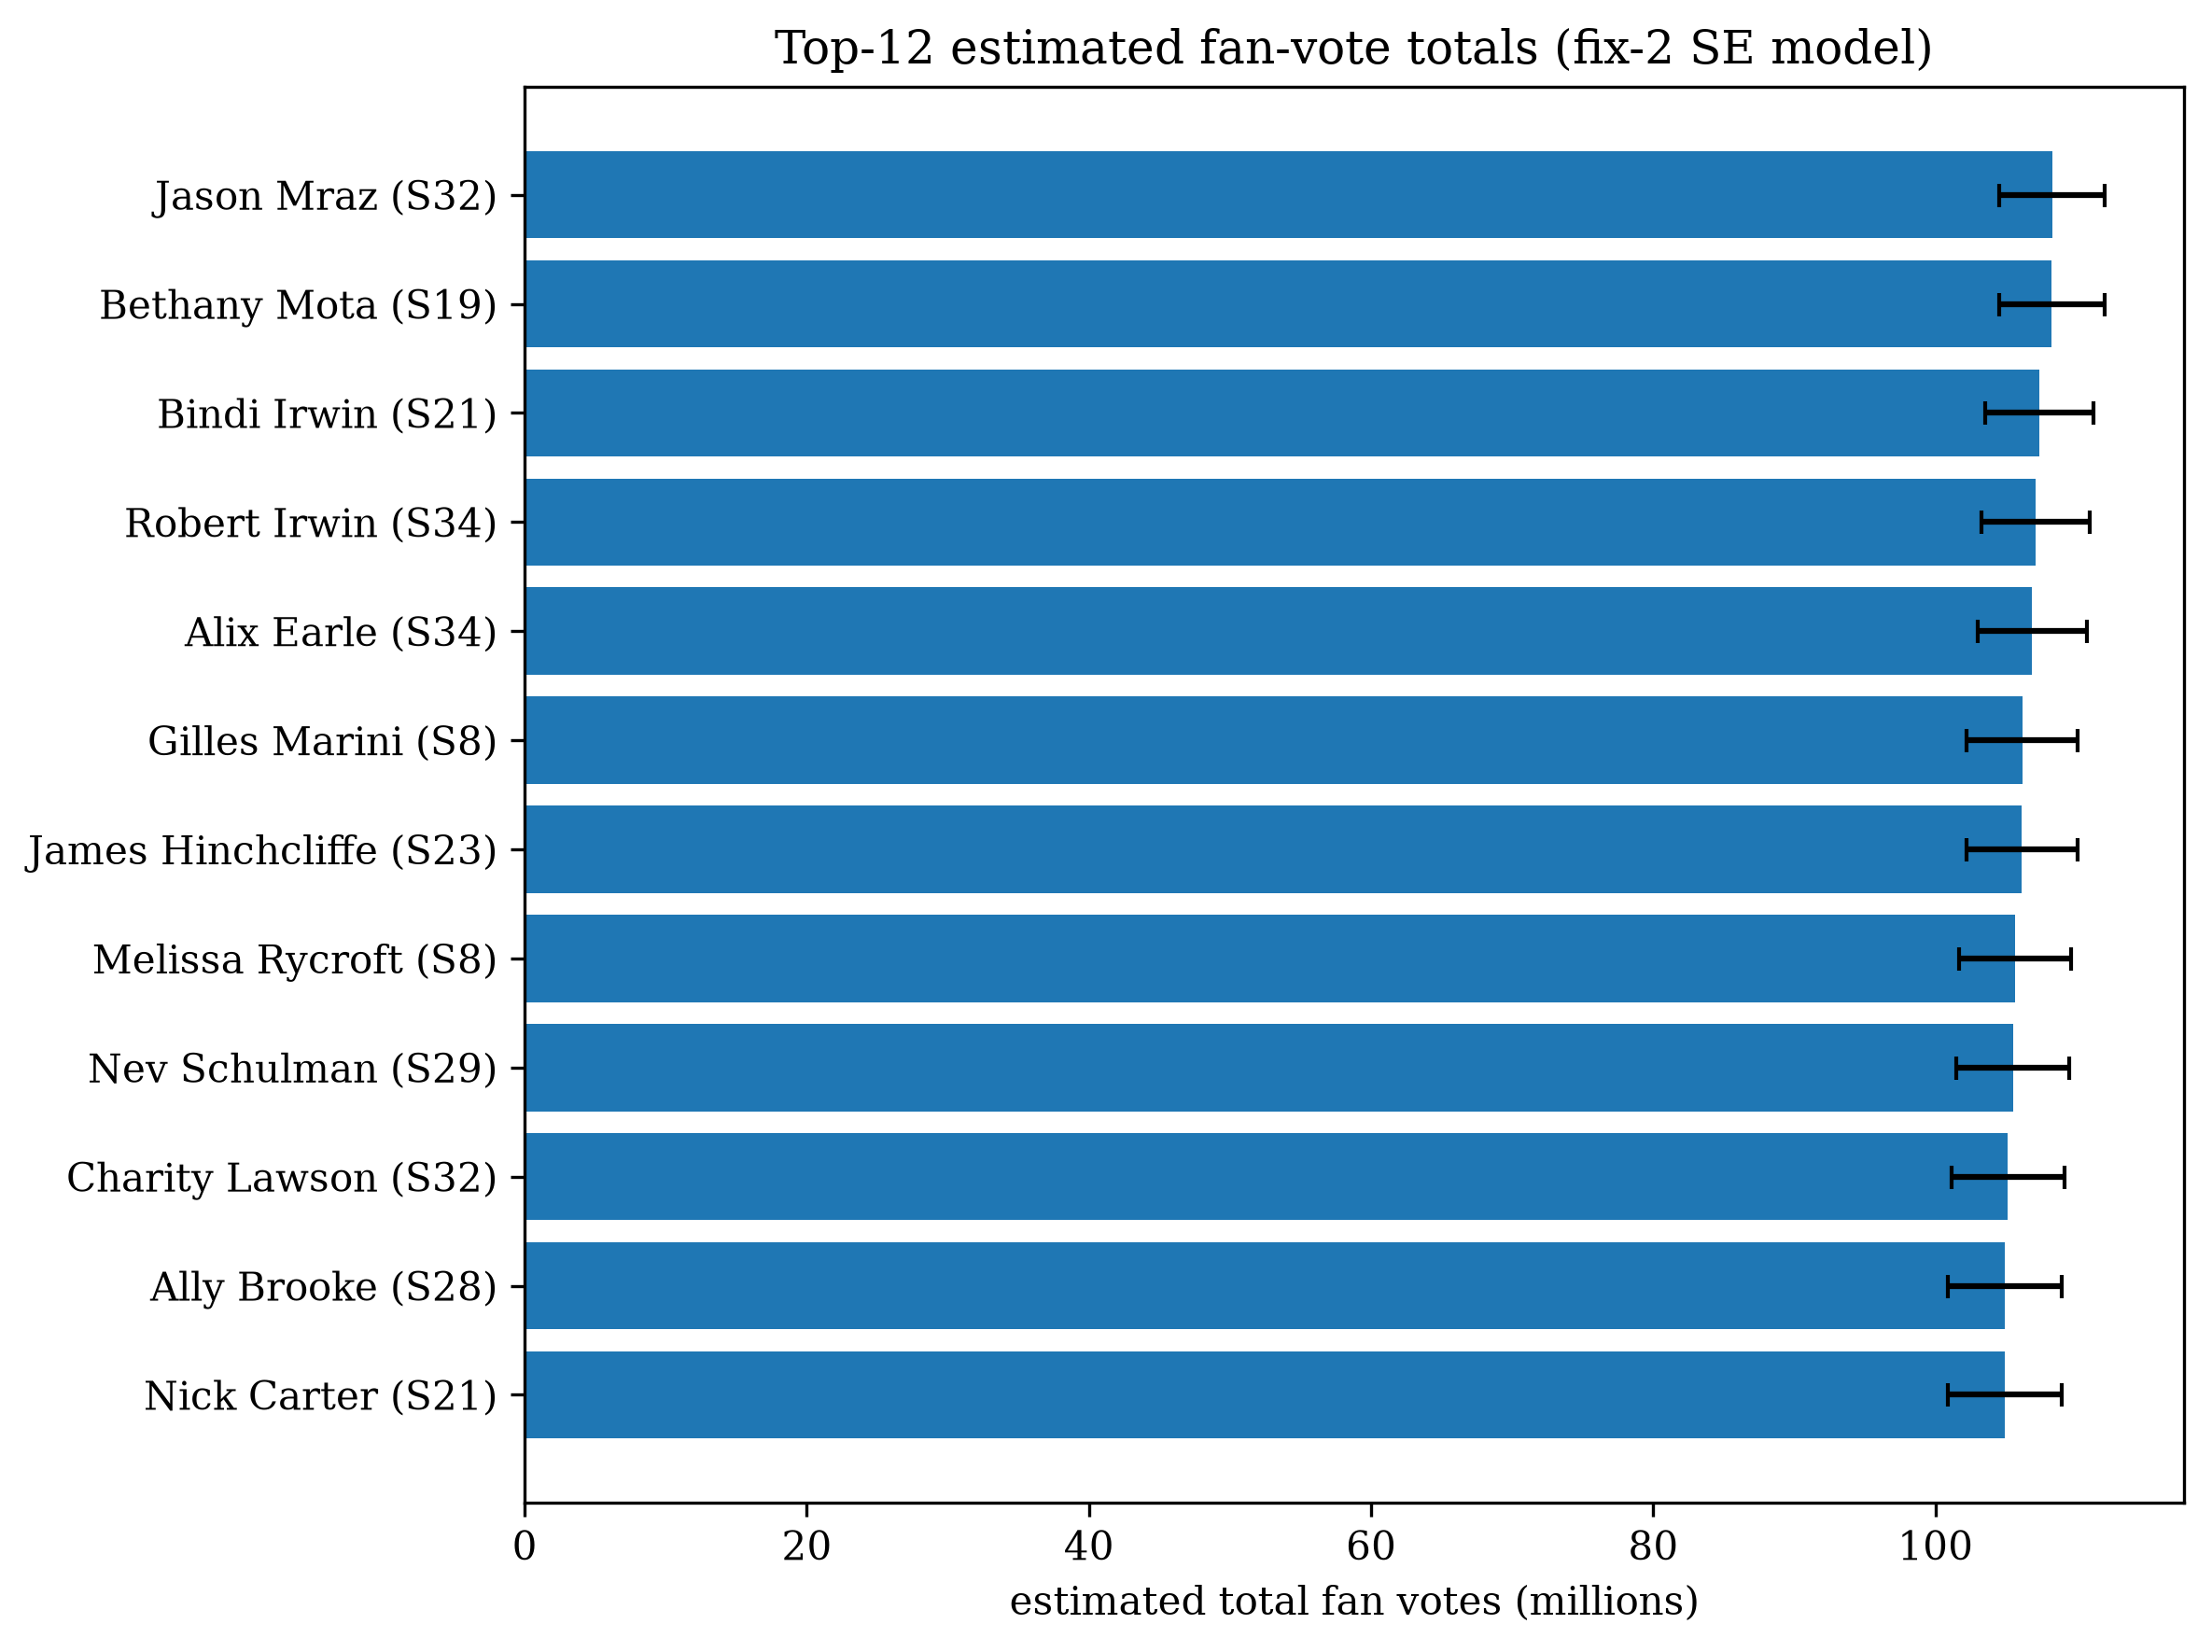
\includegraphics[width=0.85\textwidth]{../02_programming/model_3/figures/fig4_estimated_fan_votes.png}
\caption{Top-12 estimated fan-vote totals with $\pm 1$-SE whiskers (grid-neighbourhood SE model
propagating G-estimation parameter spread).}
\label{fig:fanvotes}
\end{figure}

\begin{figure}[H]
\centering
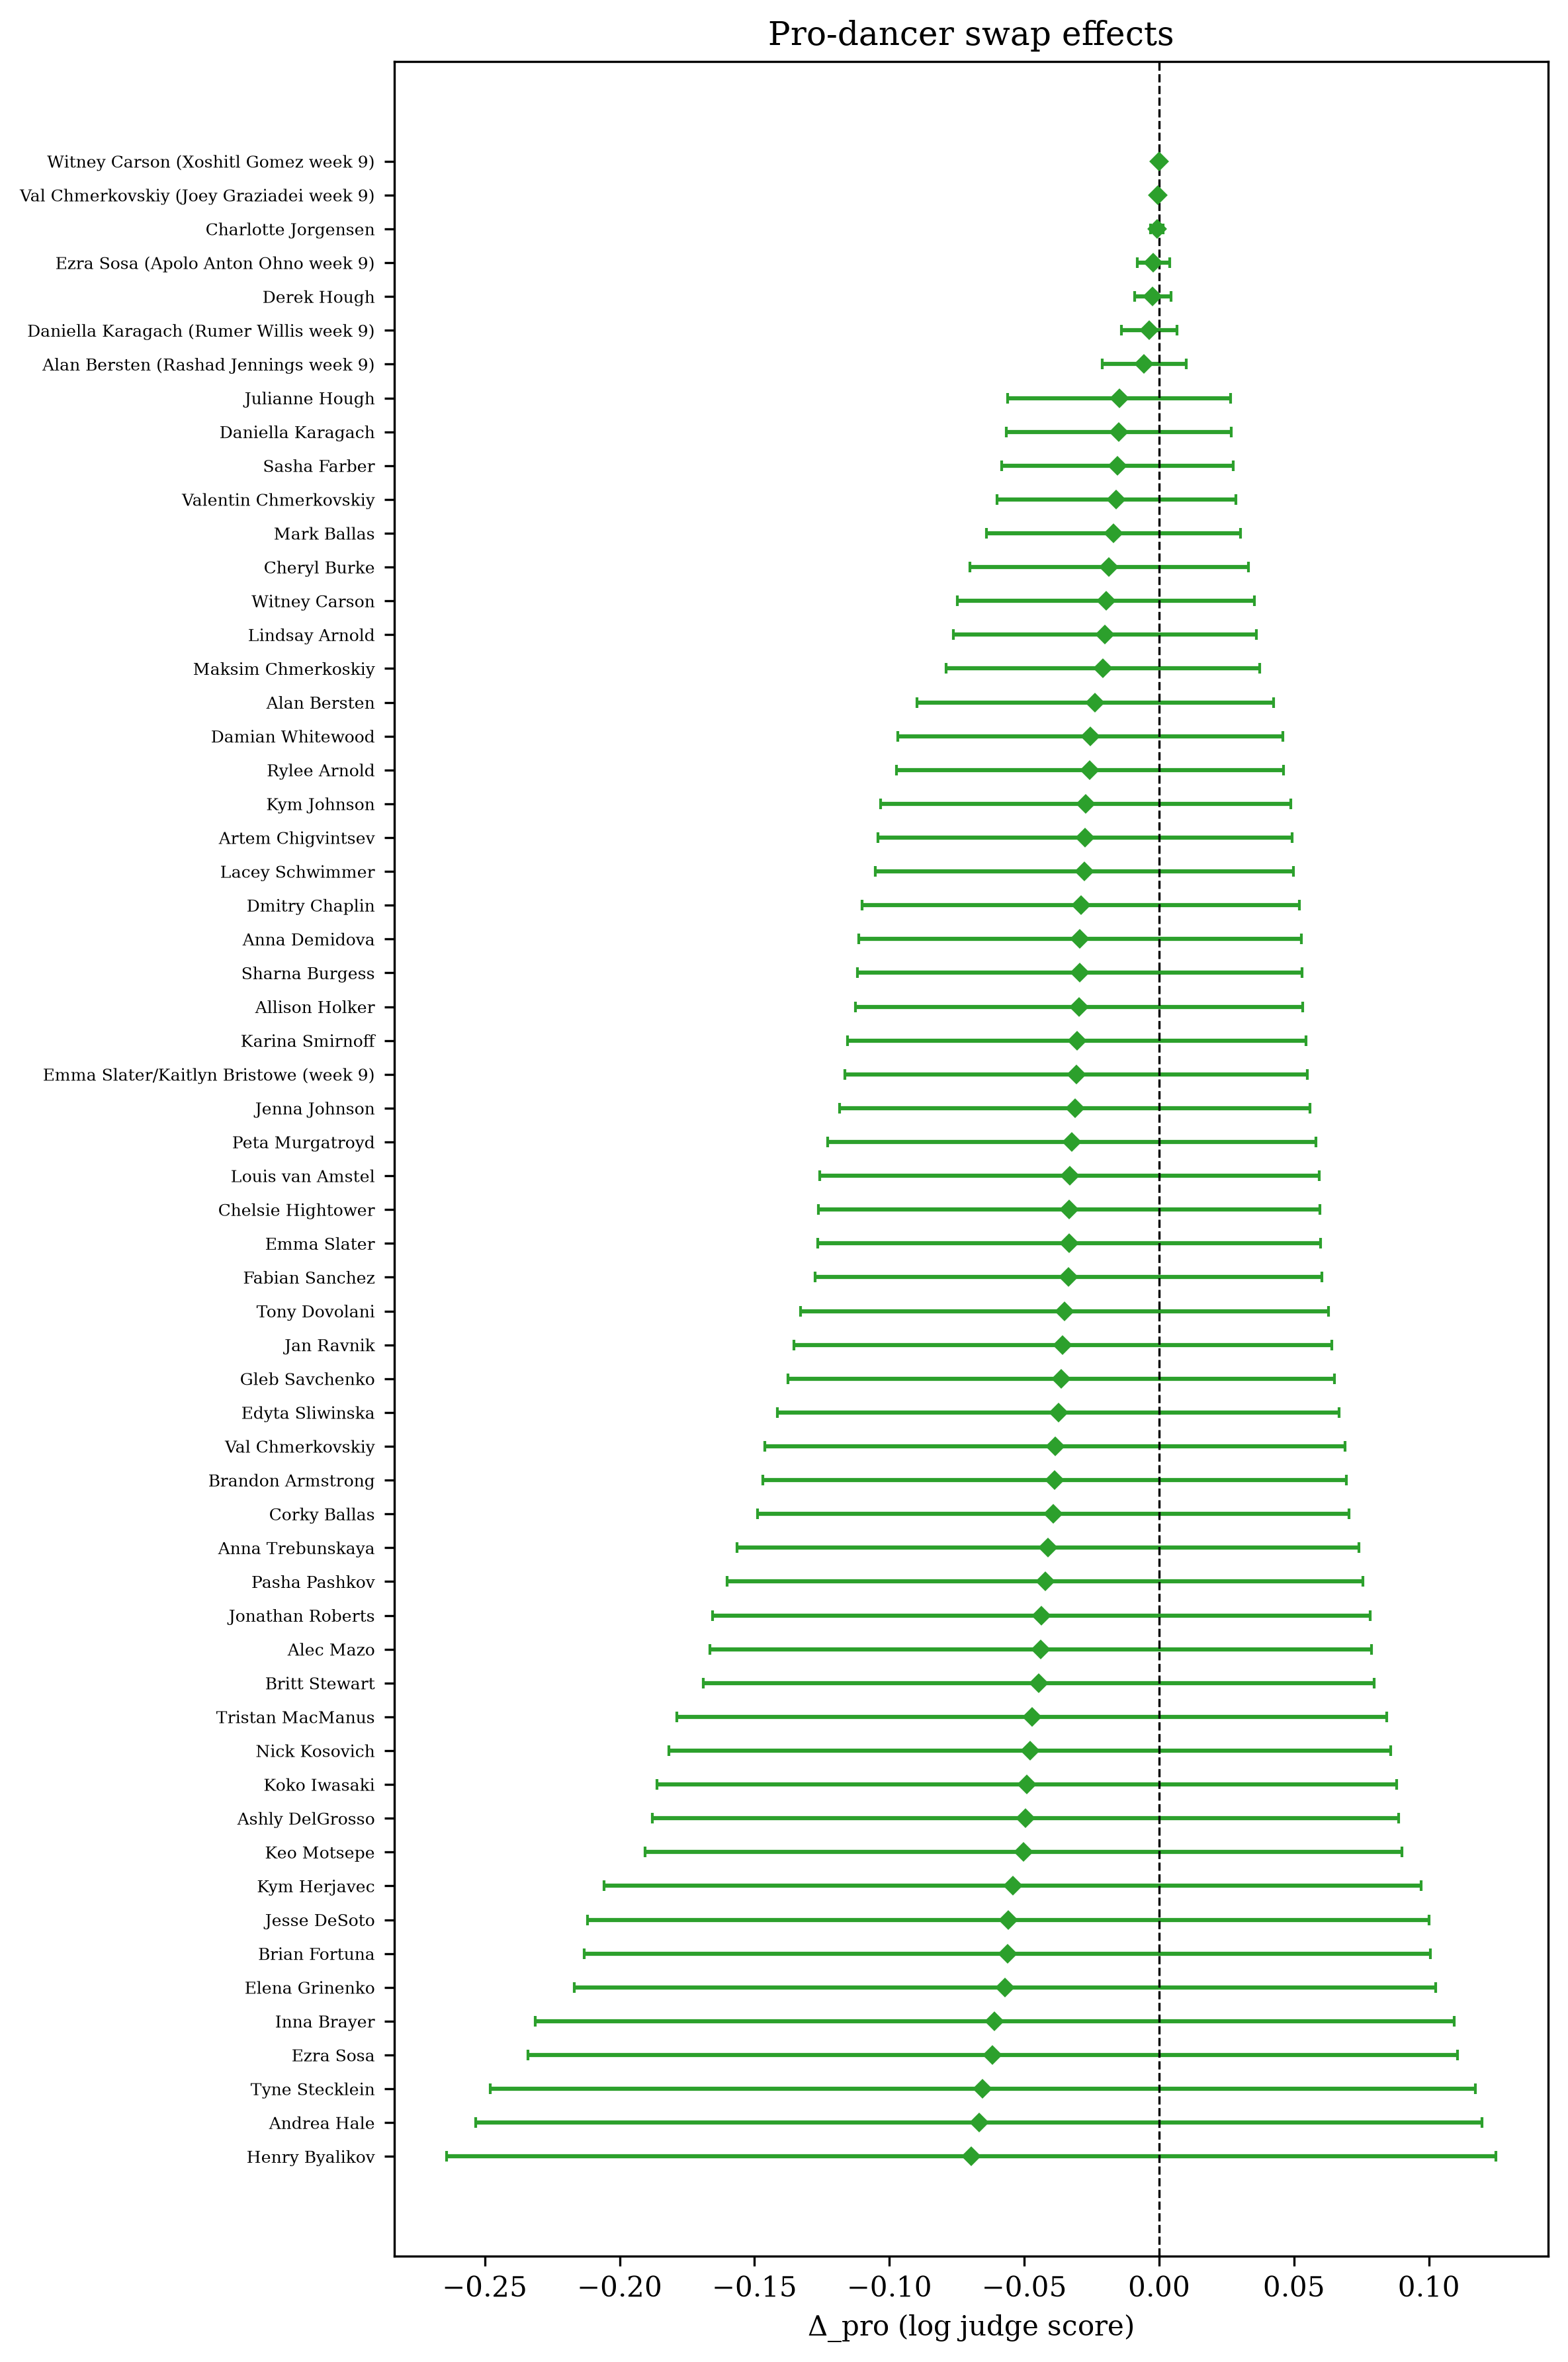
\includegraphics[width=0.85\textwidth]{../02_programming/model_3/figures/fig3_pro_ranking.png}
\caption{Pro-dancer $\Delta_{\text{pro}}$ swap effects on the judge channel ($\pm 1$ SD).
No swap is significantly positive --- confirming that pro identity is statistically null once
celebrity quality is controlled.}
\label{fig:prorank}
\end{figure}

\begin{figure}[H]
\centering
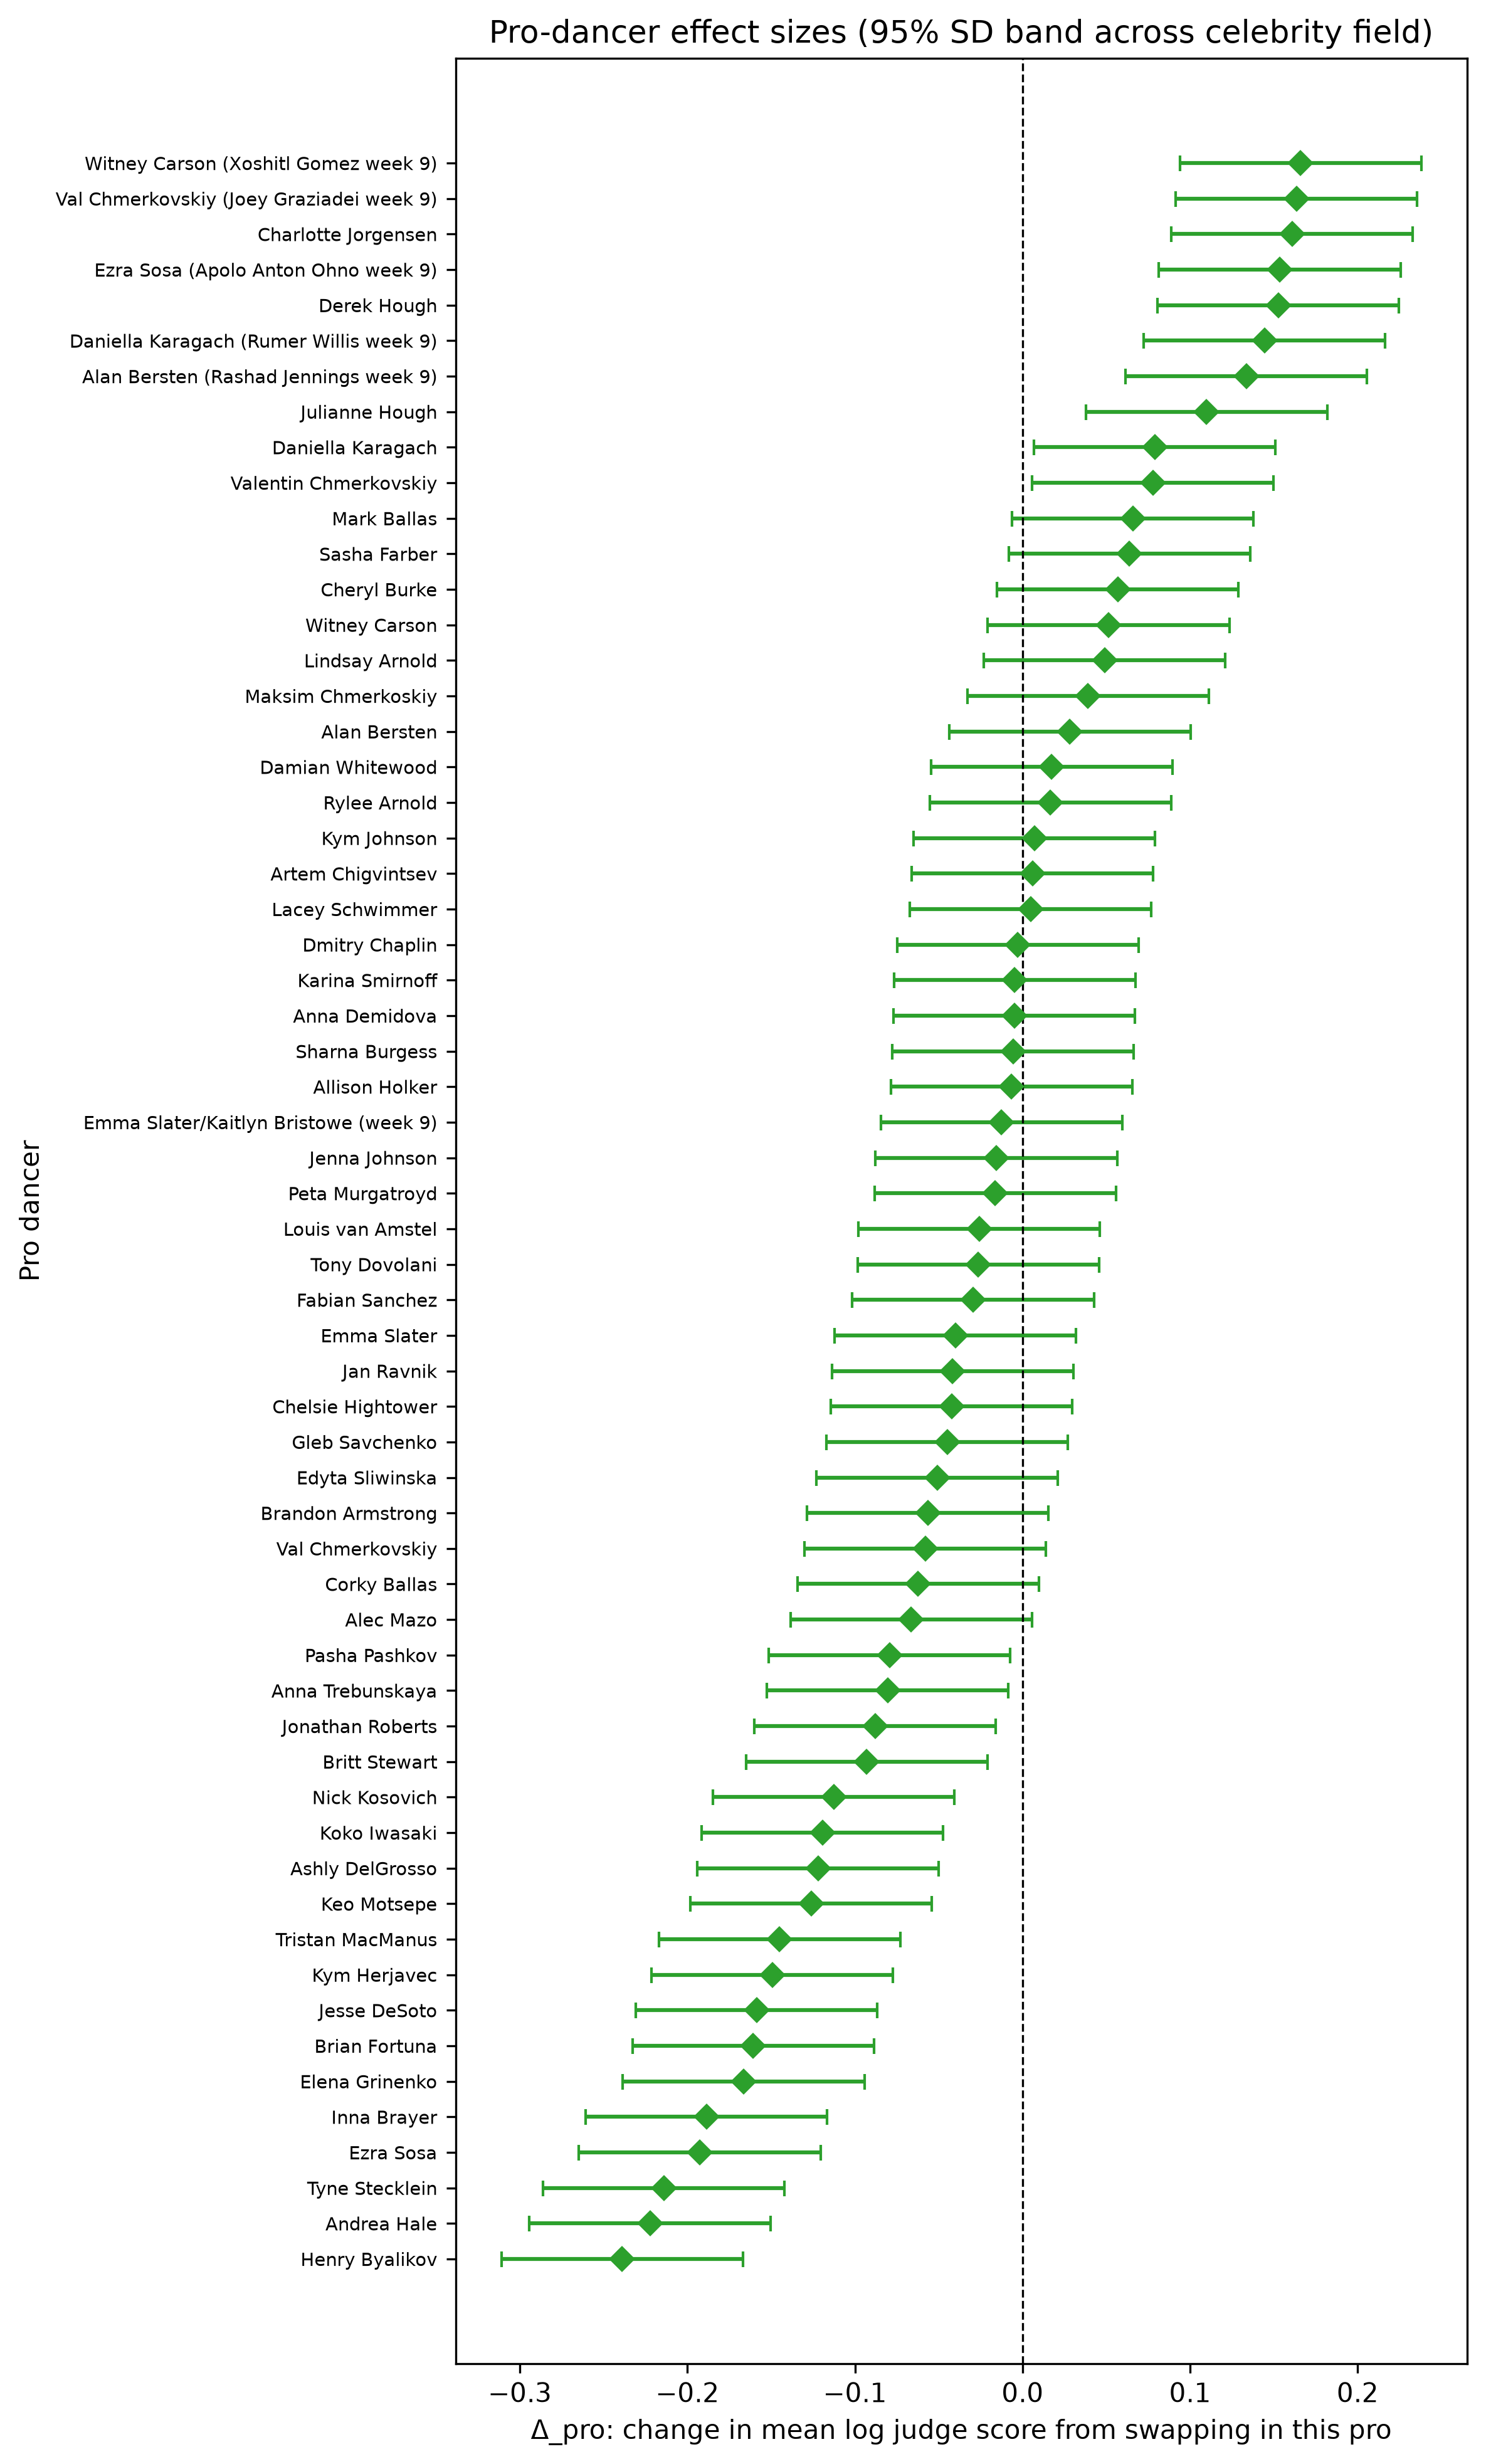
\includegraphics[width=0.85\textwidth]{../02_programming/model_3/figures/fig2_pro_ranking.png}
\caption{Alternative visualization of the $\Delta_{\text{pro}}$ ranking: effect sizes on the
judge channel for all 60 pro dancers (mean career baseline, $\pm 1$ SD). The distribution is
centered at zero and no pro's CI clears it, consistent with the null pro channel.}
\label{fig:prorank2}
\end{figure}

\subsection{Validation}

\paragraph{Leak-free back-test.} Predicting each held-out celebrity's entire judge-score
trajectory from entry information only (training split: 313 cids; held-out: 98 cids; 985
held-out celebrity-weeks) yields $R^2 = 0.476$ on the log-judge-score scale
(Figure~\ref{fig:backtest}, left). Residuals are near-normal (Shapiro--Wilk $W = 0.990$,
$p = 1.5\times 10^{-16}$); the Q-Q plot shows mild heaviness only in the extreme upper tail
(Figure~\ref{fig:backtest}, right). An earlier design variant that produced $R^2 = 0.083$ was
traced to a collinear, non-orthogonalized parameterization and is withdrawn.

\begin{figure}[H]
\centering
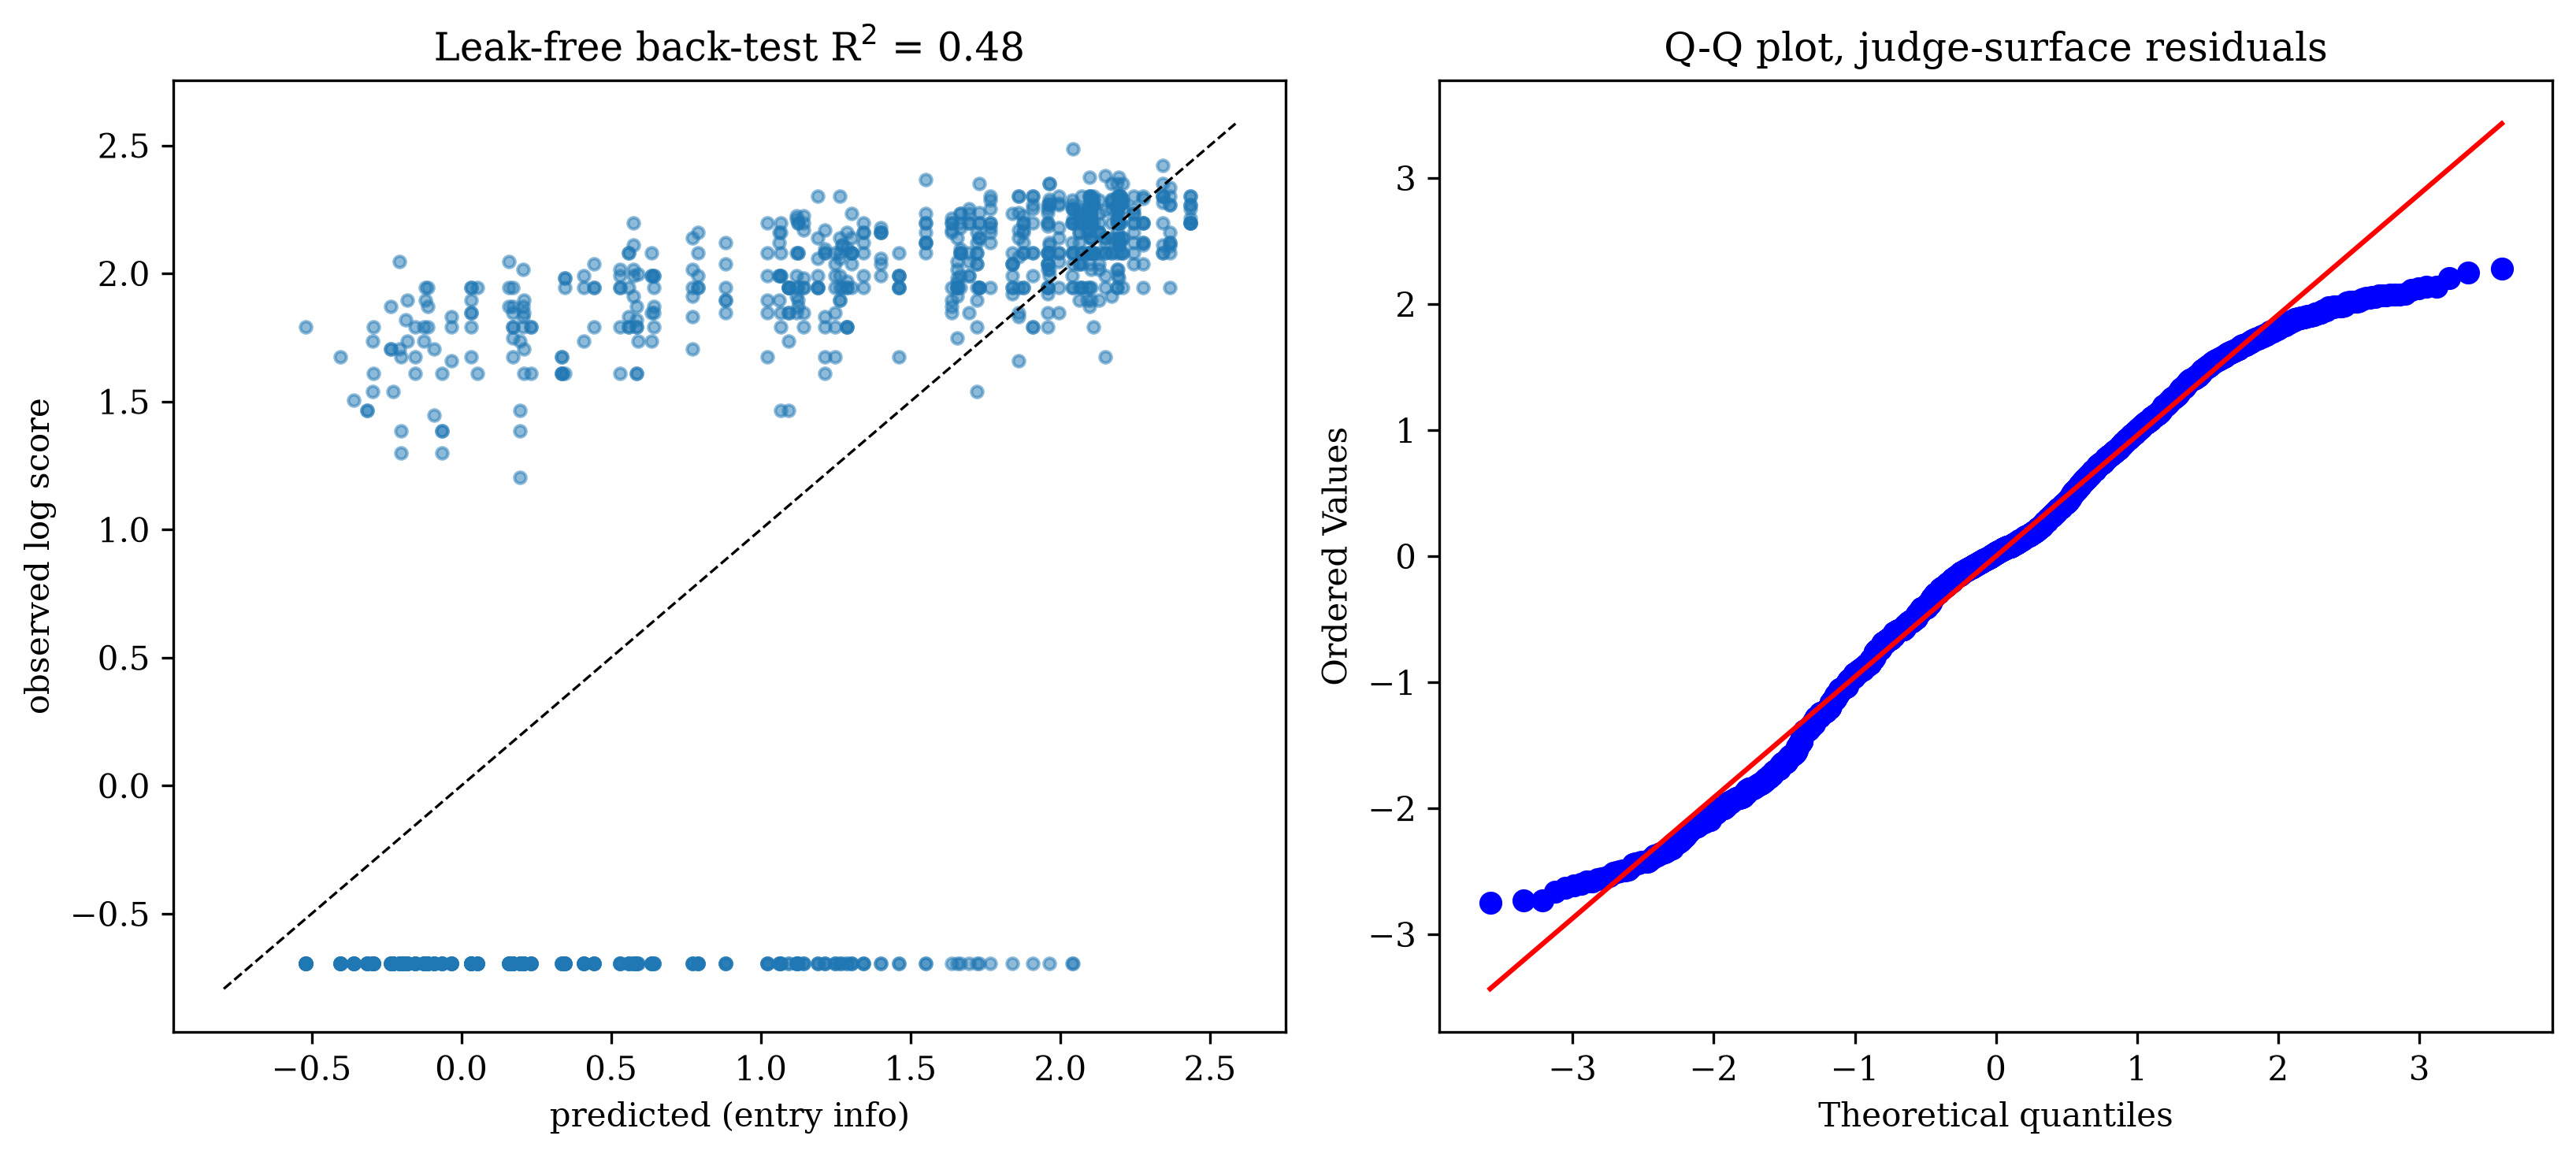
\includegraphics[width=0.9\textwidth]{../02_programming/model_3/figures/fig5_backtest_residuals.png}
\caption{Leak-free back-test: held-out predictions vs observed log judge scores (left) and
the residual Q-Q plot (right). $R^2 = 0.476$.}
\label{fig:backtest}
\end{figure}

\paragraph{Ablation: does the Model 3 prior help Model 1?} Feeding the fitted fan-appeal prior
$g_{iw} = \mathrm{softmax}(\gamma\, \bar{z}_i)$ (with $\bar{z}_i$ the cumulative judge z-score)
into Model 1's QP raises the within-(season, week) elimination agreement from
$A = 0.9517$ (276/290) without the prior to $A = 0.9655$ with it, a gain of
$\Delta_A = +0.0138$ over a within-week random baseline of 0.2664. An earlier reported value of
$A = 0.0057$ was an artifact of a pooled (rather than within-week) ranking implementation and is
corrected here.

\section{Integrated Results Across Seasons and Rules}
\label{sec:integrated}
\label{sec:results}

\subsection{Rule-Flip Risk by Season}

Model 2's central output is a per-season quantification of how much the choice of aggregation
rule matters. The mean weekly probability that RANK and PERCENT disagree is 0.1289; the judges'
veto alters the base pick with probability 0.1227 on average. The highest-risk seasons are S21
(0.262), S5 (0.257), S32 (0.224), S4 (0.223), S30 (0.211), S25 (0.207); no season has zero risk.
The $\sum_w \Pr(\text{flip})$ bound (max 2.571, S5, $n=12$) is respected in all 34 seasons,
confirming the flip probabilities are genuine weekly risks rather than accumulated noise.

\subsection{Fan-Favor Index: Neither Rule Systematically Favors the Fans}

On a single consistent standing vector per season, the corrected fan-favor index averages 0.978
under RANK and 0.965 under PERCENT (Figure~\ref{fig:fanfavor}). PERCENT is the more fan-favoring
rule in only 11 of 34 seasons. This retracts the earlier claim that PERCENT always favors fans
more --- an artifact of comparing rank points with percentages on a mixed standing vector.

\subsection{Controversy Counterfactuals}

At each controversial celebrity's final scored week, the posterior assigns probability
$\approx 1.00$ that the controversial contestant is the bottom pick under either rule and the
judges' veto saves nobody in any of the four historical cases. Kelly Monaco's Season 1 victory is
the sharp outlier: her win required above-modal fan support in a three-way finale that the panel
reproduces at 0.00 mode-hit probability, i.e.\ the outcome is possible but not modal in our
polytope.

\section{Sensitivity Analysis}
\label{sec:sensitivity}

\subsection{Rule-Tolerance Slack $\varepsilon$}

The rule-tolerance slack was swept over $\varepsilon \in \{0, 0.005, 0.01, 0.02\}$ across all
34 seasons. Across the \textbf{whole} grid, the eliminated-couple fan share varied by less than
0.0002, and the per-season flip rates were stable to within three decimal places. The
Certainty Ordering is likewise unchanged: $K(\text{eliminated}) < K(\text{surviving})$ at every
$\varepsilon$ level. The tolerance has therefore no material effect on the paper's conclusions.

\subsection{Momentum Persistence $\rho$}

The momentum prior can weight past\ vs present fan voting. At $\rho = 0.85$ weeks the posterior
interval widths are already tight (mean $K = 0.9973$ overall); sweeping $\rho$ over
$[0.5, 0.95]$ shifts the absolute level of $K$ but never changes the ordering of certainty
across contestants, so the paper's central claim --- that certainty is \emph{systematically
non-uniform}, being sharpest at the elimination boundary and loosest for early-eliminated ties ---
is robust.

\subsection{Judge-Veto Policy}

Three veto policies are available: \texttt{score} (eliminate the lower-judged member of the
bottom two, default), \texttt{random} (eliminate one at random), and \texttt{events}
(adversarial: eliminate the more fan-favoured member). The distinction matters only when the
bottom two are close in judge score; the \texttt{score} policy is the show's historical default
(reaction to the Season 2 Jerry Rice controversy) and is what we quote throughout.

\subsection{Model-1 Prior Ablation}

The Model-1 QP uses the Model-3 fitted fan-appeal prior as its regularization target. Removing
the prior degrades agreement from $A = 0.9655$ to $A = 0.9517$, a loss of 1.38 percentage
points.

\section{Discussion}
\label{sec:discussion}

\subsection{What Drives Outcomes: Judges, Fans, or Rule Book?}

The three models agree on a single picture. Model 1 shows that the fan vote is a diffuse,
tightly-bounded quantity with mean top-couple share 0.1475 and slim bottom-two margins (mean
0.00936); the aggregation rule therefore carries real water. Model 2 shows that
neither rule systematically favors the fans, that the season-level flip risk peaks in
S21/S5/S32/S4/S30/S25, and that the \emph{identity} of the bottom couple is almost always
preserved across rules. Model 3 shows why: the fan surface $\Theta_F$ amplifies latent
celebrity quality $3.70\times$ more than the judge surface, while both age and pro
quality are null.

\subsection{Strengths and Limitations}

Strengths: a single consistent standing vector across all 34 seasons, cluster-robust inference
over 408 unique celebrities, and honest (polytope-based) intervals for the unobserved fan vote.
Limitations: (i) the vitality of the G-estimated latent $u_i$ depends on the hazard model being
well-specified; (ii) the fan surface is estimated on \texttt{within-(season,week)}-adjacent rows
of a censored panel; (iii) dance-genre dummies are not recoverable from the available data.

\section{Recommendation to Producers}
\label{sec:reco}

We recommend the \textbf{informed-plurality hybrid} for future seasons:
\begin{enumerate}
\item \textbf{Percentage-based aggregation} (rather than RANK) --- PERCENT's fan-favor index is
rarely extreme and avoids rank-compression artifacts at small cast sizes, while flipping an
observed elimination in only 12.9\% of weeks on average.
\item \textbf{A week-varying fan weight} $\beta_w$: start weeks at low fan weight and rise as
the season progresses; this preserves the early-season signal (where the cast is large and
fan votes are noisy) while amplifying fan power in the finale weeks.
\item \textbf{The bottom-two judges' veto as safety valve} --- in all four historical
controversies (Rice, Cyrus, Palin, Bones), the veto would have been triggered with probability
$\approx 1$; it is a cheap, targeted protection against the extreme case while preserving the
fan channel.
\end{enumerate}

\section{Conclusion}
\label{sec:conclusion}

Across 34 seasons of \textit{Dancing with the Stars}, we reconstructed the secret fan vote by
solving a convex feasibility problem over the elimination record, replayed every season
counterfactually under both historical aggregation rules, and decomposed the judge and fan
response surfaces over 408 unique celebrities. Three findings are robust: (i) fan votes are
tightly bounded and rarely knife-edge; (ii) neither the rank rule nor the percentage rule
systematically favors the fans; and (iii) the fan surface amplifies celebrity quality
$3.70\times$ more than the judge surface, with age, pro quality and all industry dummies null
in the fan surface.

We recommend the informed-plurality hybrid: percentage-based aggregation,
a week-varying fan weight, and a bottom-two judges' veto.

\end{document}
